\PassOptionsToPackage{unicode=true}{hyperref} % options for packages loaded elsewhere
\PassOptionsToPackage{hyphens}{url}
%
\documentclass[12pt,italian,]{report}
\usepackage{lmodern}
\usepackage{amssymb,amsmath}
\usepackage{ifxetex,ifluatex}
\usepackage{fixltx2e} % provides \textsubscript
\ifnum 0\ifxetex 1\fi\ifluatex 1\fi=0 % if pdftex
  \usepackage[T1]{fontenc}
  \usepackage[utf8]{inputenc}
  \usepackage{textcomp} % provides euro and other symbols
\else % if luatex or xelatex
  \usepackage{unicode-math}
  \defaultfontfeatures{Ligatures=TeX,Scale=MatchLowercase}
\fi
% use upquote if available, for straight quotes in verbatim environments
\IfFileExists{upquote.sty}{\usepackage{upquote}}{}
% use microtype if available
\IfFileExists{microtype.sty}{%
\usepackage[]{microtype}
\UseMicrotypeSet[protrusion]{basicmath} % disable protrusion for tt fonts
}{}
\IfFileExists{parskip.sty}{%
\usepackage{parskip}
}{% else
\setlength{\parindent}{0pt}
\setlength{\parskip}{6pt plus 2pt minus 1pt}
}
\usepackage{hyperref}
\hypersetup{
            pdftitle={Progetto Usabilità e User Experience 2018/2019},
            pdfauthor={Filippo Bartolini; Adamo Fapohunda; Giacomo Leidi; Cristian Castiglione},
            pdfborder={0 0 0},
            breaklinks=true}
\urlstyle{same}  % don't use monospace font for urls
\usepackage{longtable,booktabs}
% Fix footnotes in tables (requires footnote package)
\IfFileExists{footnote.sty}{\usepackage{footnote}\makesavenoteenv{longtable}}{}
\usepackage{graphicx,grffile}
\makeatletter
\def\maxwidth{\ifdim\Gin@nat@width>\linewidth\linewidth\else\Gin@nat@width\fi}
\def\maxheight{\ifdim\Gin@nat@height>\textheight\textheight\else\Gin@nat@height\fi}
\makeatother
% Scale images if necessary, so that they will not overflow the page
% margins by default, and it is still possible to overwrite the defaults
% using explicit options in \includegraphics[width, height, ...]{}
\setkeys{Gin}{width=\maxwidth,height=\maxheight,keepaspectratio}
\setlength{\emergencystretch}{3em}  % prevent overfull lines
\providecommand{\tightlist}{%
  \setlength{\itemsep}{0pt}\setlength{\parskip}{0pt}}
\setcounter{secnumdepth}{0}
% Redefines (sub)paragraphs to behave more like sections
\ifx\paragraph\undefined\else
\let\oldparagraph\paragraph
\renewcommand{\paragraph}[1]{\oldparagraph{#1}\mbox{}}
\fi
\ifx\subparagraph\undefined\else
\let\oldsubparagraph\subparagraph
\renewcommand{\subparagraph}[1]{\oldsubparagraph{#1}\mbox{}}
\fi

% set default figure placement to htbp
\makeatletter
\def\fps@figure{htbp}
\makeatother

\ifnum 0\ifxetex 1\fi\ifluatex 1\fi=0 % if pdftex
  \usepackage[shorthands=off,main=italian]{babel}
\else
  \usepackage{polyglossia}
  \setmainlanguage[]{italian}
\fi

\title{Progetto Usabilità e User Experience 2018/2019}
\author{Filippo Bartolini \and Adamo Fapohunda \and Giacomo Leidi \and Cristian Castiglione}
\date{}

\begin{document}
\maketitle

{
\setcounter{tocdepth}{2}
\tableofcontents
}
\newpage
\section{Introduzione}\label{introduzione}
Kids Experience è un applicativo web legato al sito madre Kiabi.

Kiabi è un'azienda francese di e-commerce e distribuzione di
abbigliamento pronto moda, facente parte del gruppo Mulliez. Il suo
slogan \emph{``La moda a piccoli prezzi''} si basa su prodotti a prezzi
accessibili per tutta la famiglia.

Kids Experience offre ai clienti la possibilità di personalizzare
autonomamente megliette per bambini e ragazzi, da 3 a 12 anni, ampliando la vasta gamma di prodotti offerti da Kiabi.

Il punto di forza di questa nuova categoria di prodotti è costituito dall'estrema personalizzazione di magliette per bambini offerta all'utente.

\section{Ricerca etnografica}\label{ricerca-etnografica}
È possibile subito osservare come i bisogni che Kids Experience andrà a soddisfare non si trovino nei primi livelli della gerarchia di Maslow, ma si identifichino nel livello intermedio della gerarchia: il livello
di \emph{appartenenza}.

Successivamente si è fatta un'analisi del mercato dell'abbigliamento, analizzando alcuni competitors attraverso dati reperiti online.
Precisamente, come si evince dalla Fig \ref{abbigliamo_generico}, per quanto riguarda il
mercato italiano il maggiore esponente è risultato essere Zara, mentre Kiabi si posiziona al terzo posto.

\begin{figure}[h]
\centering
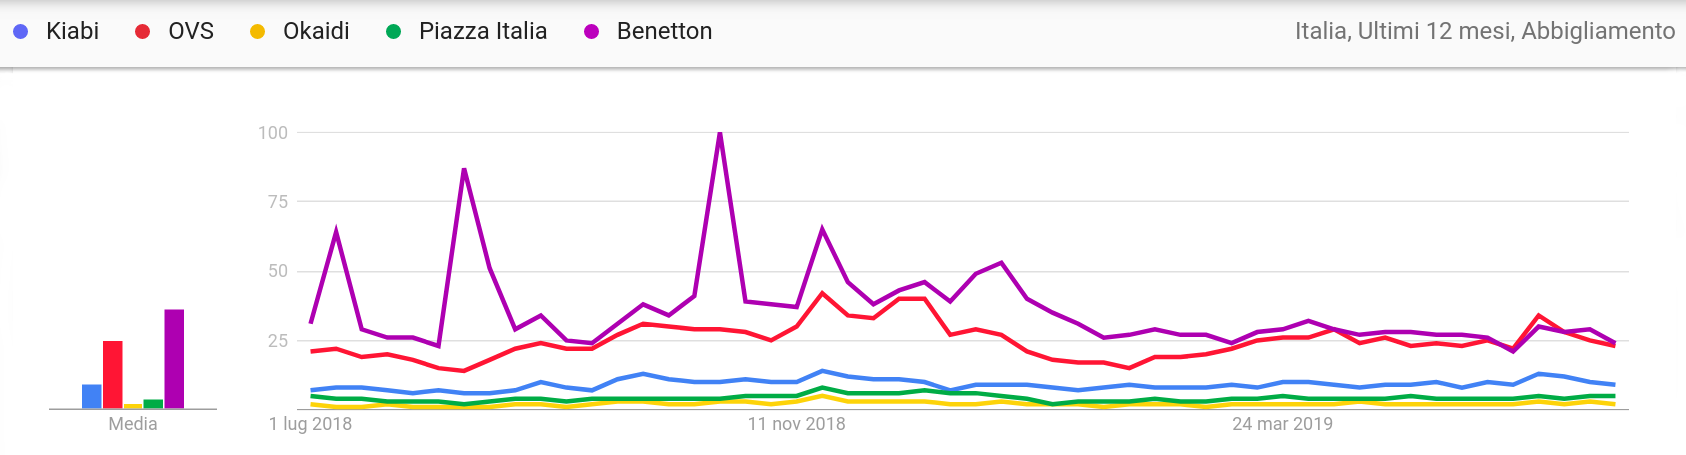
\includegraphics{img/abbigliamento_generico.png}
\caption{Ricerca di mercato - abbigliamento}
\label{abbigliamo_generico}
\end{figure}

Per quanto riguarda il mercato dell'abbigliamento da bambino, Kiabi perde un ulteriore posizione passando dal terzo al quarto posto, come mostrato in Fig. \ref{abbigliamento_bambino}.

\begin{figure}[h]
\centering
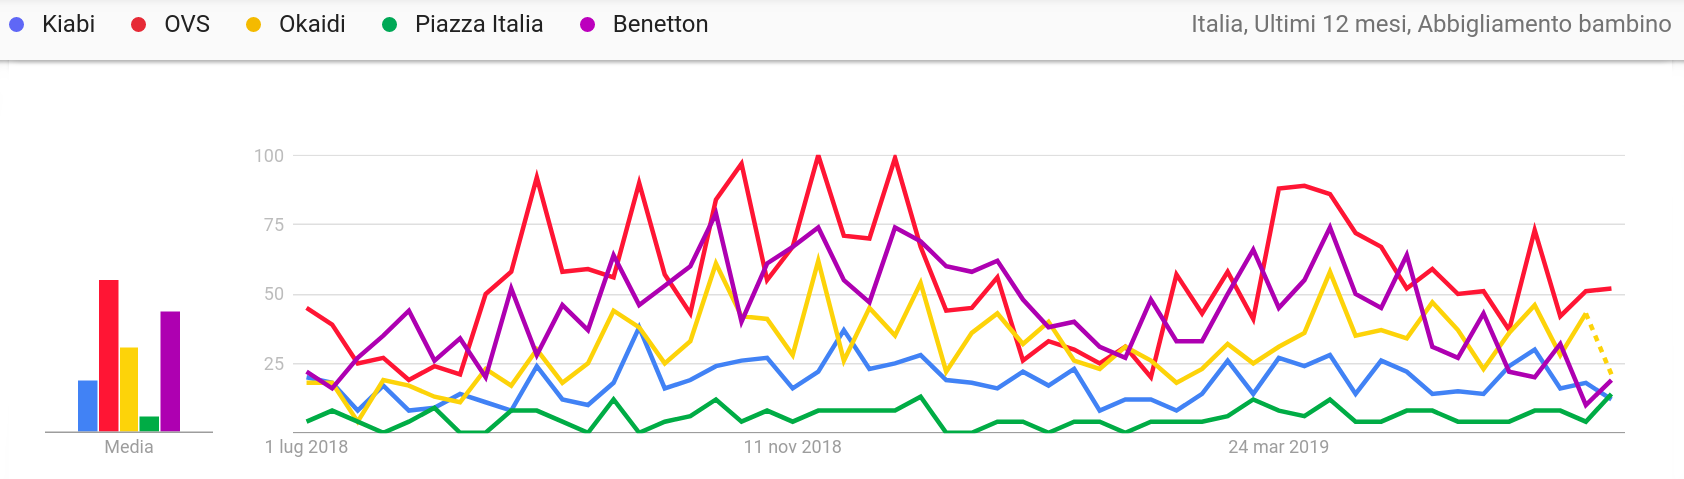
\includegraphics{img/abbigliamento_bambino.png}
\caption{Ricerca di mercato - abbigliamento bambino}
\label{abbigliamento_bambino}
\end{figure}

Dopo un'attenta analisi abbiamo deciso di prendere Kiabi come azienda madre, con l'obiettivo di rilanciarla sul mercato dell'abbigliamento per bambina/o tramite l'aggiunta di nuove features da noi ideate e proposte al Project Manager Mulliez.

L'idea di progettare magliette estremamente perzonalizzabili solo per bambini, nasce dalla semplicità del capo dettati dai minimi vincoli fisici (i.e. taglia) del target. Questo permette di garantire all'utente un'ampia gamma di personalizzazioni senza dover complicare eccessivamente
il processo di manifattura.

\newpage
\section{Blueprint}\label{Blueprint}
Le blueprint sono semplici diagrammi che definiscono l'organizzazione dei contenuti e come le varie componenti interagiscono tra di loro.

Saranno presentate quattro blueprint che mostrano rispettivamente:

\begin{enumerate}
\def\labelenumi{\arabic{enumi}.}
\tightlist
\item
  Creazione di un nuovo modello
\item
  Organizzazione delle azioni disponibili per un utente loggato
\item
  Organizzazione delle azioni disponibili per un utente non loggato
\end{enumerate}
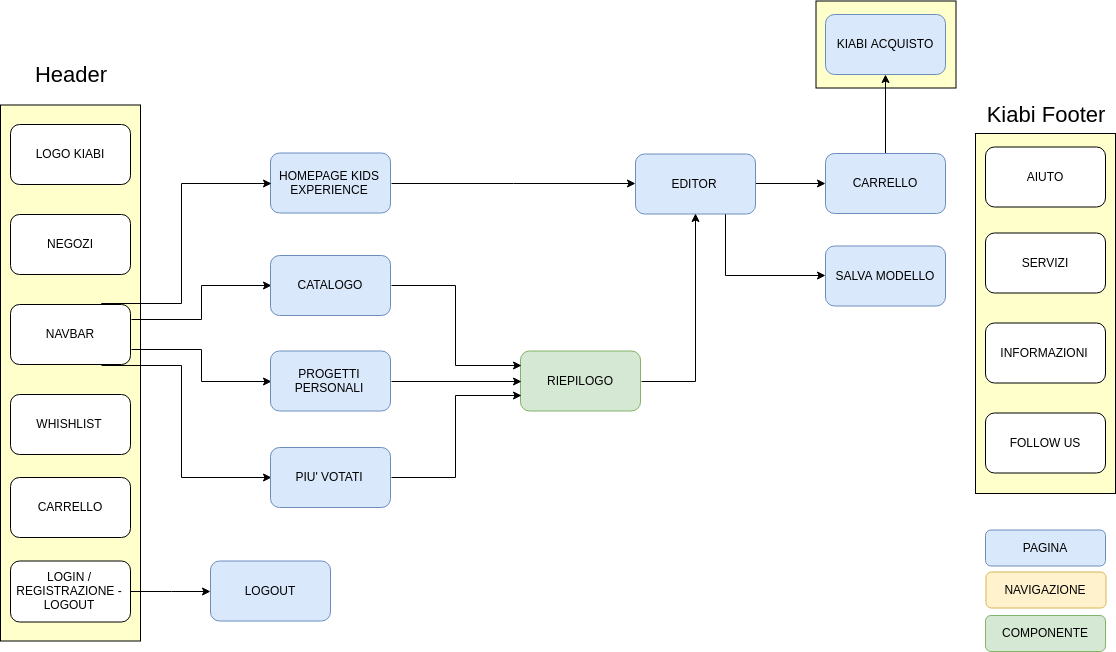
\includegraphics{blueprints/Utente_loggato.png}
\\
\\
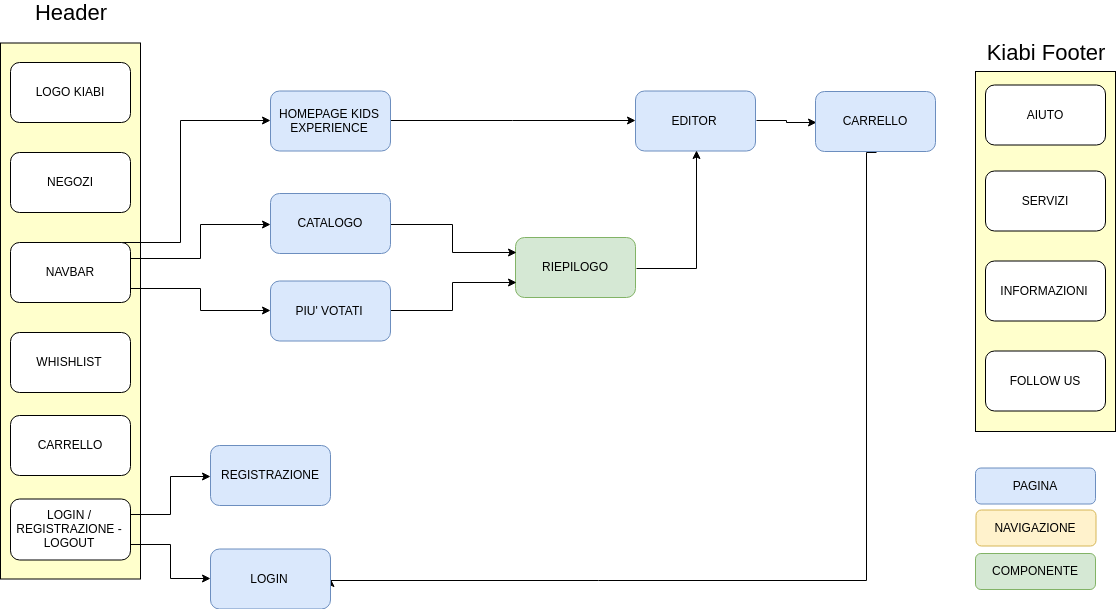
\includegraphics{blueprints/Utente_non_loggato.png}
\\
\\
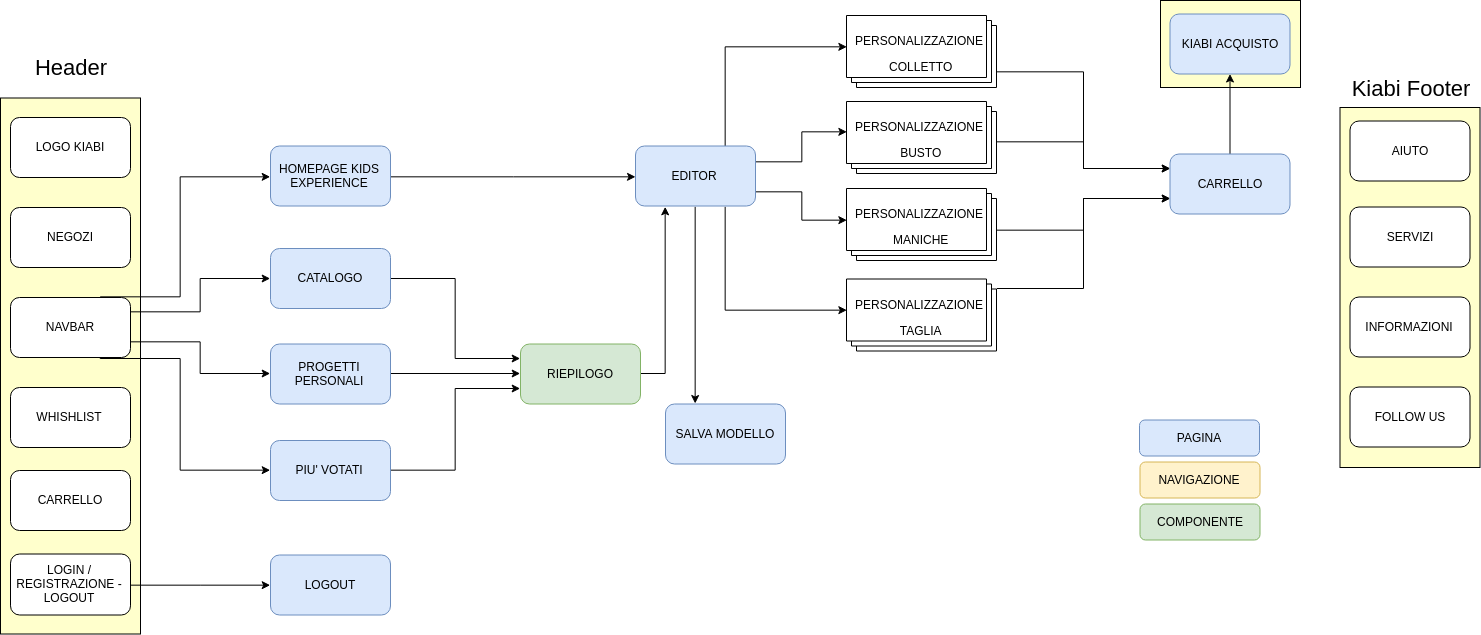
\includegraphics{blueprints/Creazione_modello.png}
\newpage
\section{Wireframes}\label{Wireframes}

\subsection{Home Kiabi}


I wireframe in Fig. \ref{kiabi_home} e Fig \ref{kiabi_home_selection} mostrano la homepage del sito kiabi con l'aggiunta dei collegamenti per raggiungere il sottosito Kids Experience.

\begin{figure}[h]
\centering
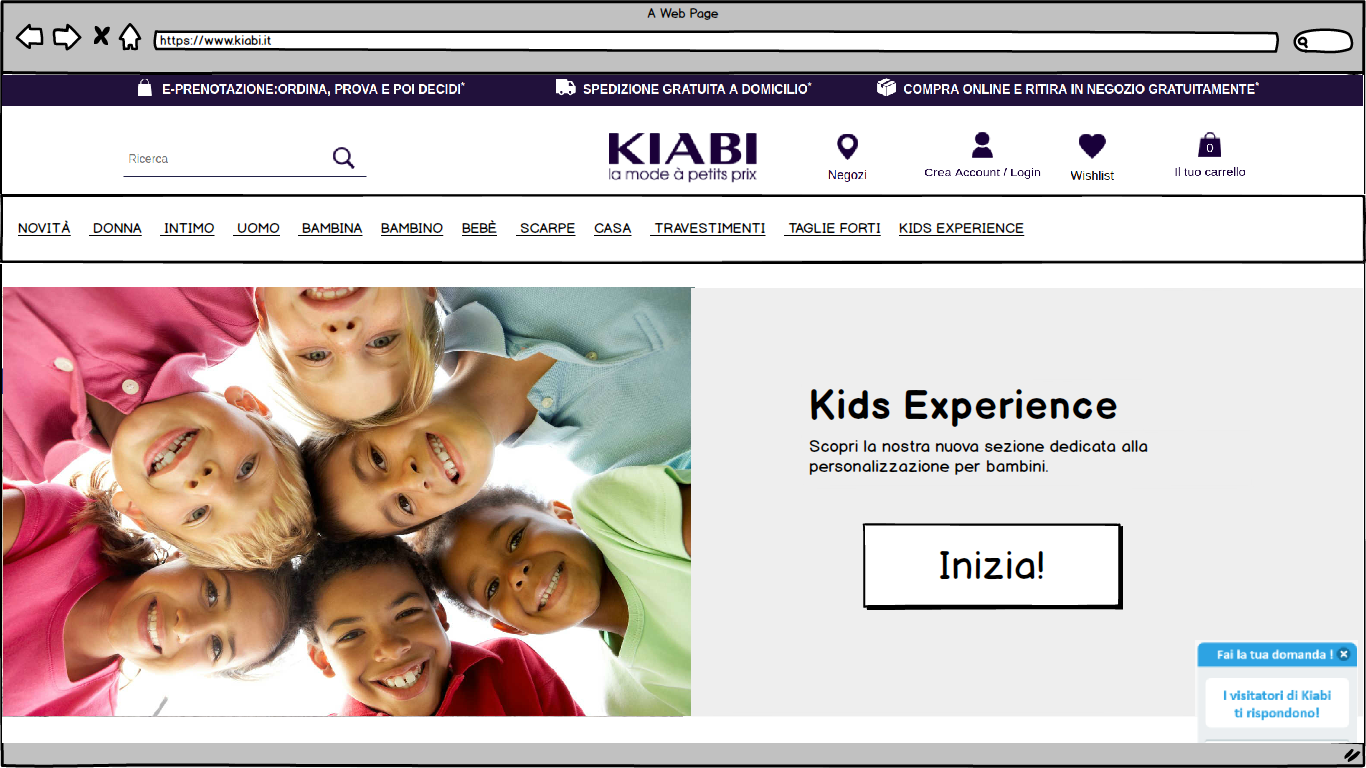
\includegraphics{balsamiq/Kiabi Home.png}
\label{kiabi_home}
\caption{Home Kiabi con link a Kids Experience}
\end{figure}

\begin{figure}[h]
\centering
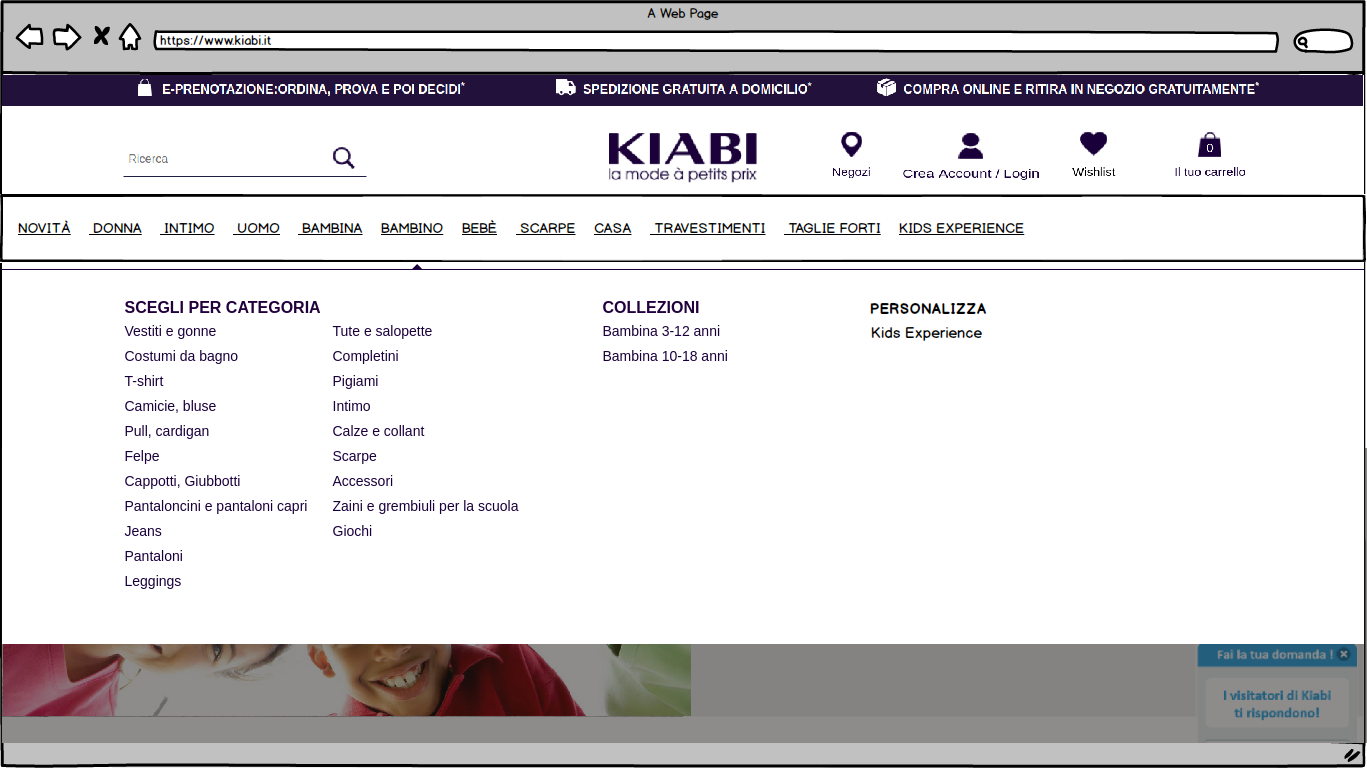
\includegraphics{balsamiq/Kiabi Scelta.png}
\label{kiabi_home_selection}
\caption{Home Kiabi - Menù bambino/a con link a Kids Experience}
\end{figure}

\subsection{Home Kids Experience} 

La home è composta da tre elementi: un header, un corpo, e un footer.
\begin{itemize}
\item
L’header rimane fisso in alto quando si scrolla la pagina, in quanto contiene elementi che possono richiedere un accesso veloce durante la visita della pagina. 
A sua volta è diviso in due sezioni. La parte in alto è identica al sito madre. La parte bassa, invece, contiene la navbar che sostituisce quella già presente nel sito kiabi.

\item
Il corpo ricopre due funzioni. 
La prima è quella di fornire un collegamento diretto all'editor corredato da reclame pubblicitaria, molto più visibile del link già presente nella navbar. 
La seconda è quella di fornire un tutorial di base sull'utilizzo dell'editor.

\item Il footer contiene elementi marginali contenenti informazioni sul sito madre kiabi.
\end{itemize}

\begin{figure}[h]
\centering
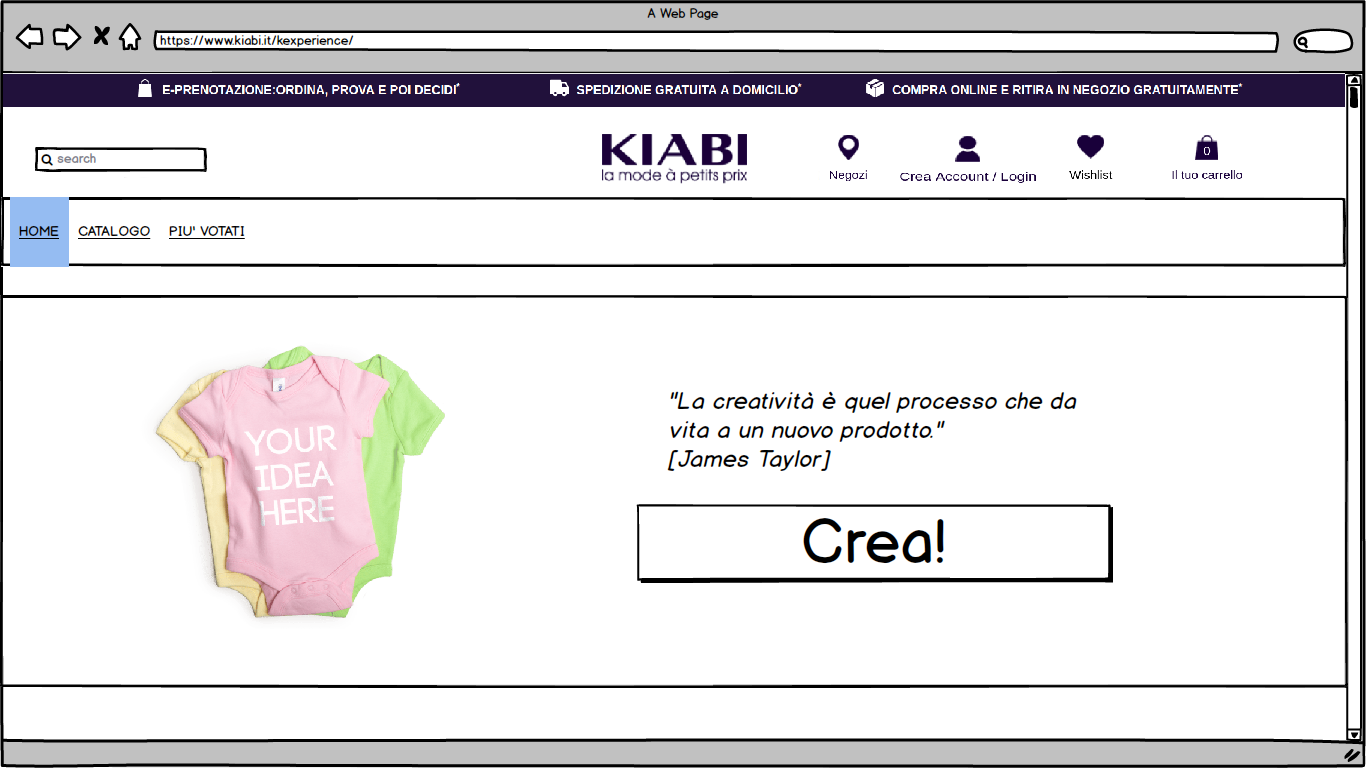
\includegraphics{balsamiq/Home Sottosito Utente Esterno .png}
\label{kids_home}
\caption{Home Kids Experience}
\end{figure}




\subsection{Catalogo} 

La sezione "Catalogo" (Fig. \ref{catalogo}) è facilmente raggiungibile a partire dalla navbar.

Questo contiene la lista dei prodotti di kids Experience ordinati per data di creazione. Tramite la searchbar è possibile effettuare ricerche in linguaggio naturale. E' possible cercare per autore, nome, colore e taglia. Aggiungendo attributi come "bottoni colletto" verrà effettuata una query per ricercare un tutti i prodotti che contengono quel tag nella lista di personalizzazioni.

Con un click su una maglietta è possibile visionare i dettagli di questa: la lista delle modifiche, l'autore e il prezzo. Dal modale (Fig. \ref{catalogo_dettagli}) è anche possibile modificare il prodotto entrando nell'editor.

Facendo over con il mouse su una maglietta, compaiono i due tasti di like/dislike più il tasto condividi. Mentre la condivisione è sempre possibile, la funzionalità di votazione tramite like/dislike è disabilitata per l'utente che non ha effettuato il login. In tal caso compare il messaggio visibile in Fig. \ref{catalogo_non_loggato}.


\begin{figure}[h]
\centering
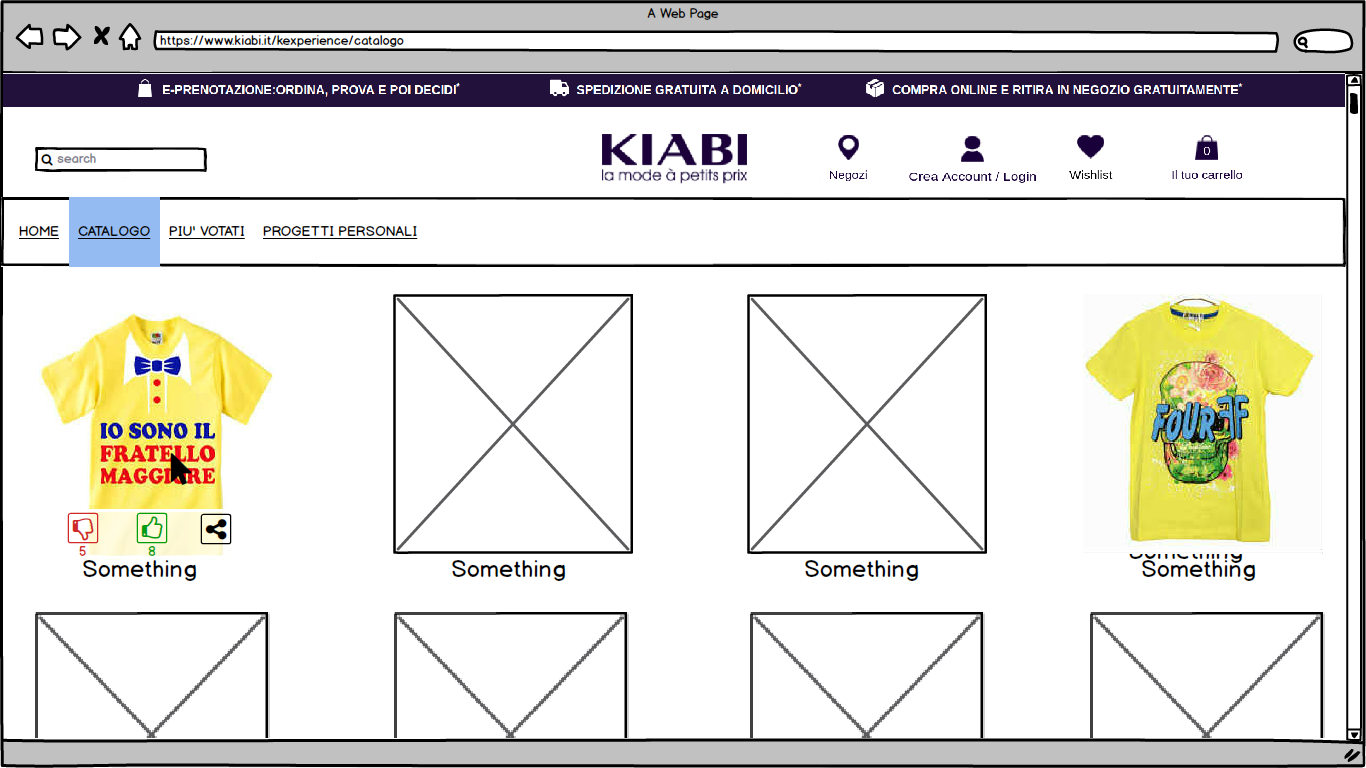
\includegraphics{balsamiq/Catalogo.png}
\label{catalogo}
\caption{Sezione Catalogo}
\end{figure}

\begin{figure}[h]
\centering
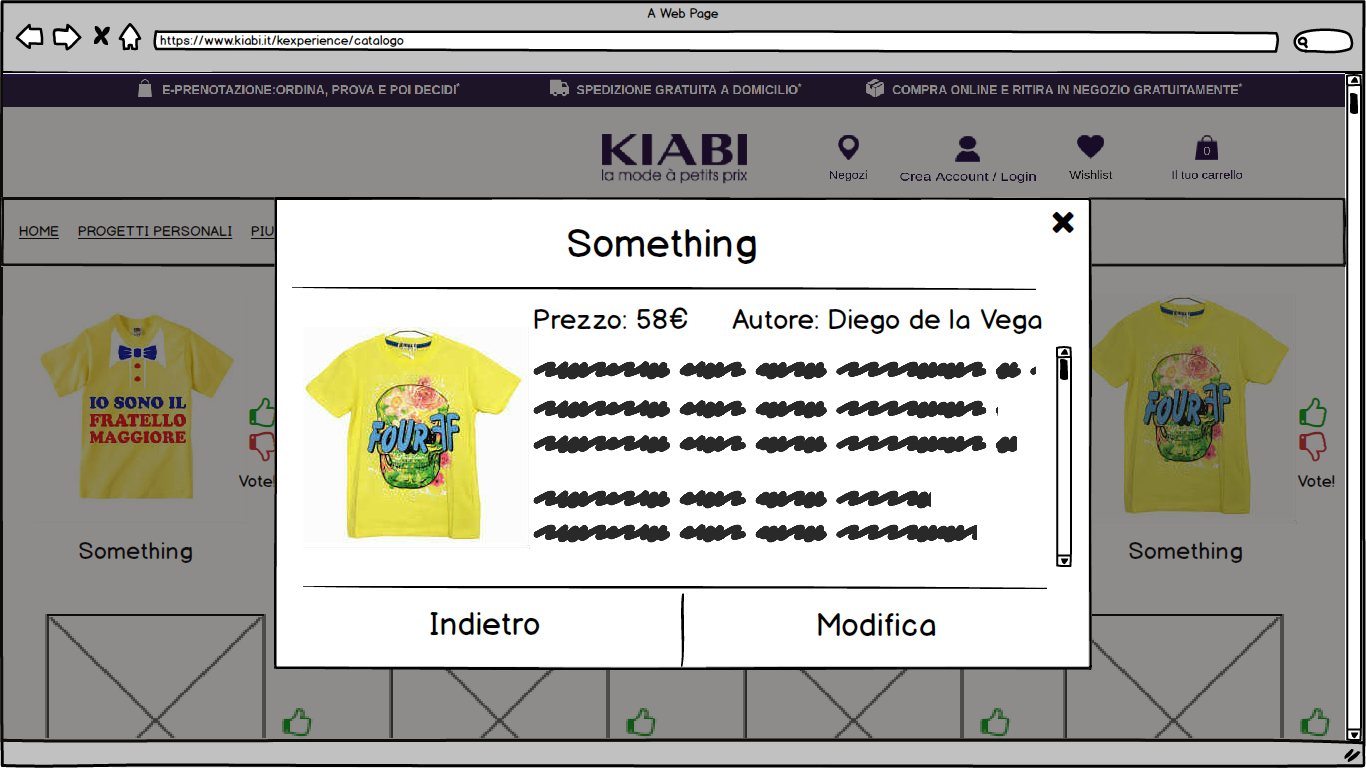
\includegraphics{balsamiq/Catalogo details.png}
\label{catalogo_dettagli}
\caption{Sezione Catalogo - Dettagli prodotto}
\end{figure}

\begin{figure}[h]
\centering
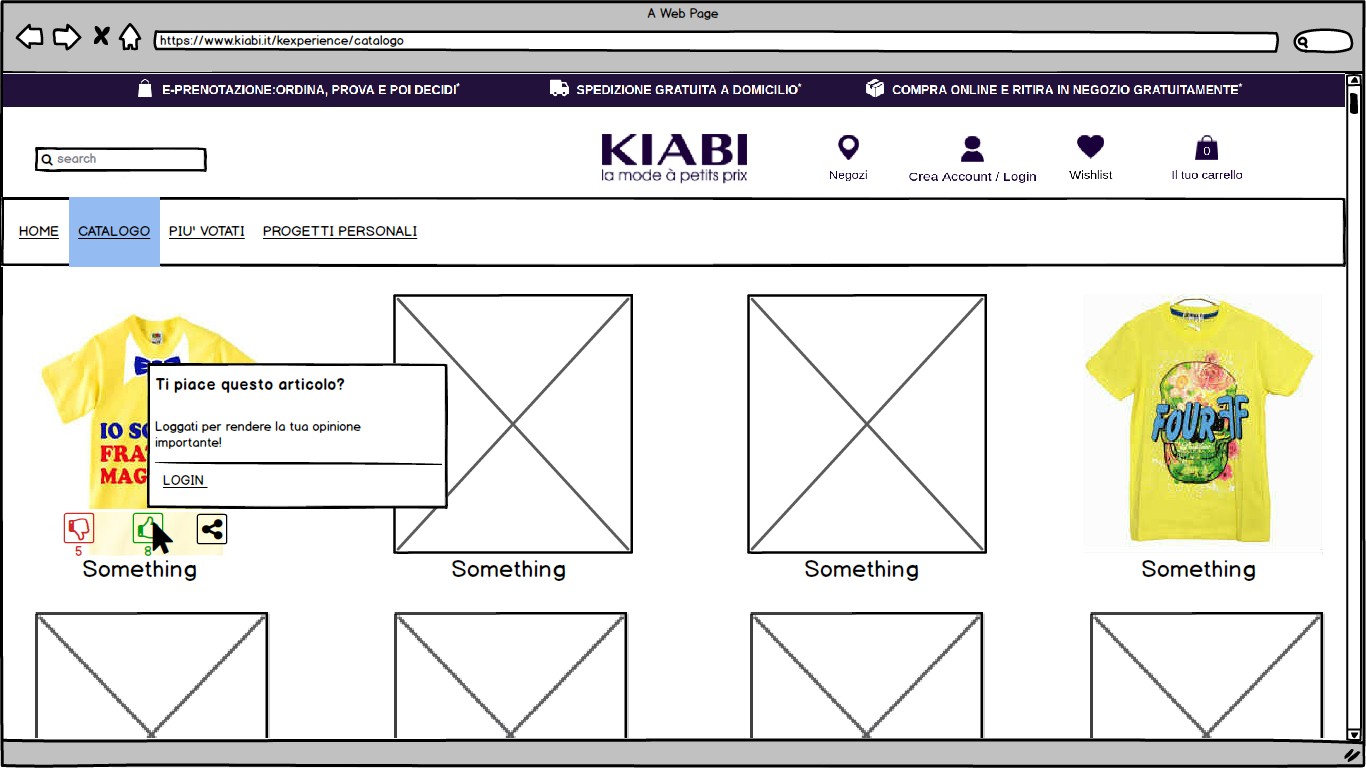
\includegraphics{balsamiq/Catalogo login.png}
\label{catalogo_non_loggato}
\caption{Sezione Catalogo - Utente non loggato}
\end{figure}

\subsection{Progetti Personali} 

La sezione progetti personali contiene la lista dei prodotti customizzati dall'utente. Tale sezione è accessible solo dopo che un utente ha effettuato il login.

Come nella sezione catalogo, anche in questo caso è possibile accedere ai dettagli del prodotto con un click.

Facendo over viene data la possiblità di votare (like/dislike), condividere ed eliminare un prodotto. In quest'ultimo caso viene mostrato un modale all'utente un modale per rendere l'operazione più macchinosa in quanto irreversibile.

\begin{figure}[h]
\centering
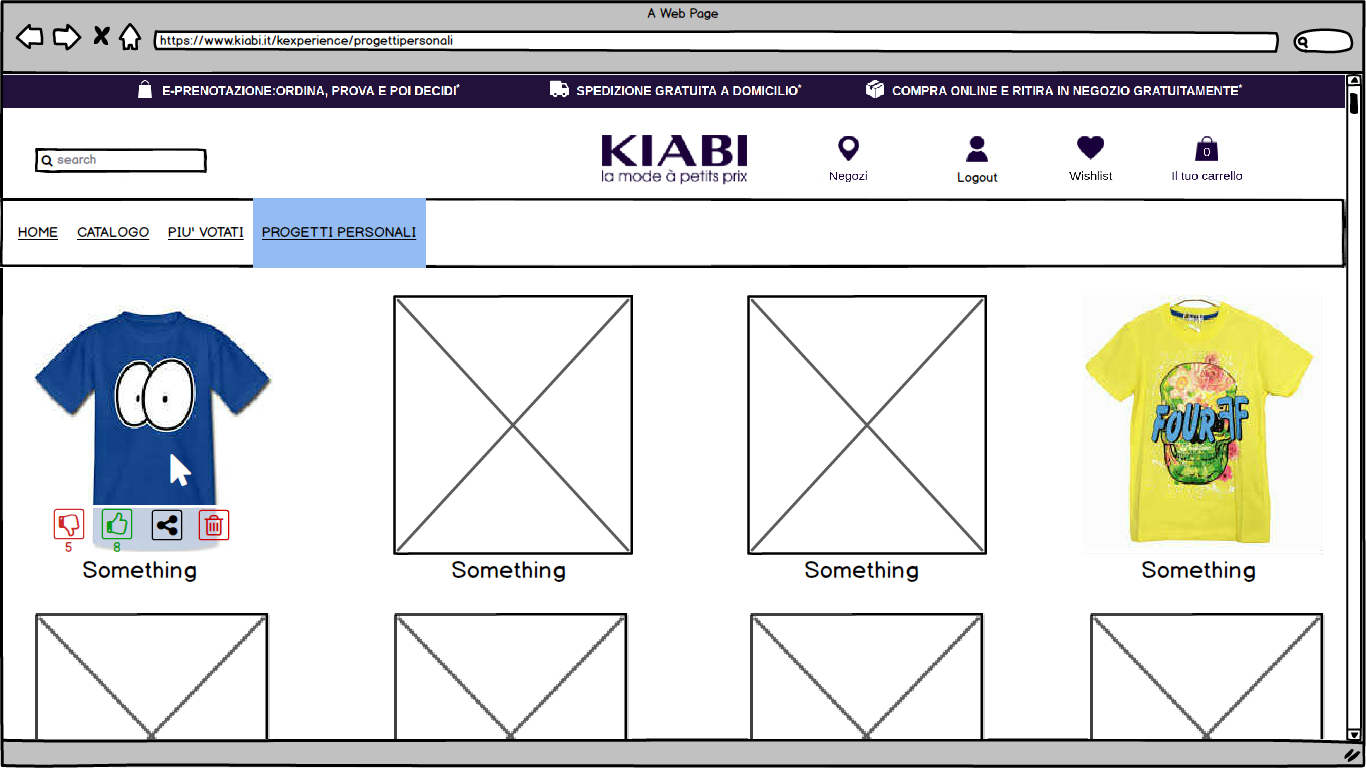
\includegraphics{balsamiq/Progetti Personali.png}
\label{progetti_personali}
\caption{Progetti Personali}
\end{figure}


\begin{figure}[h]
\centering
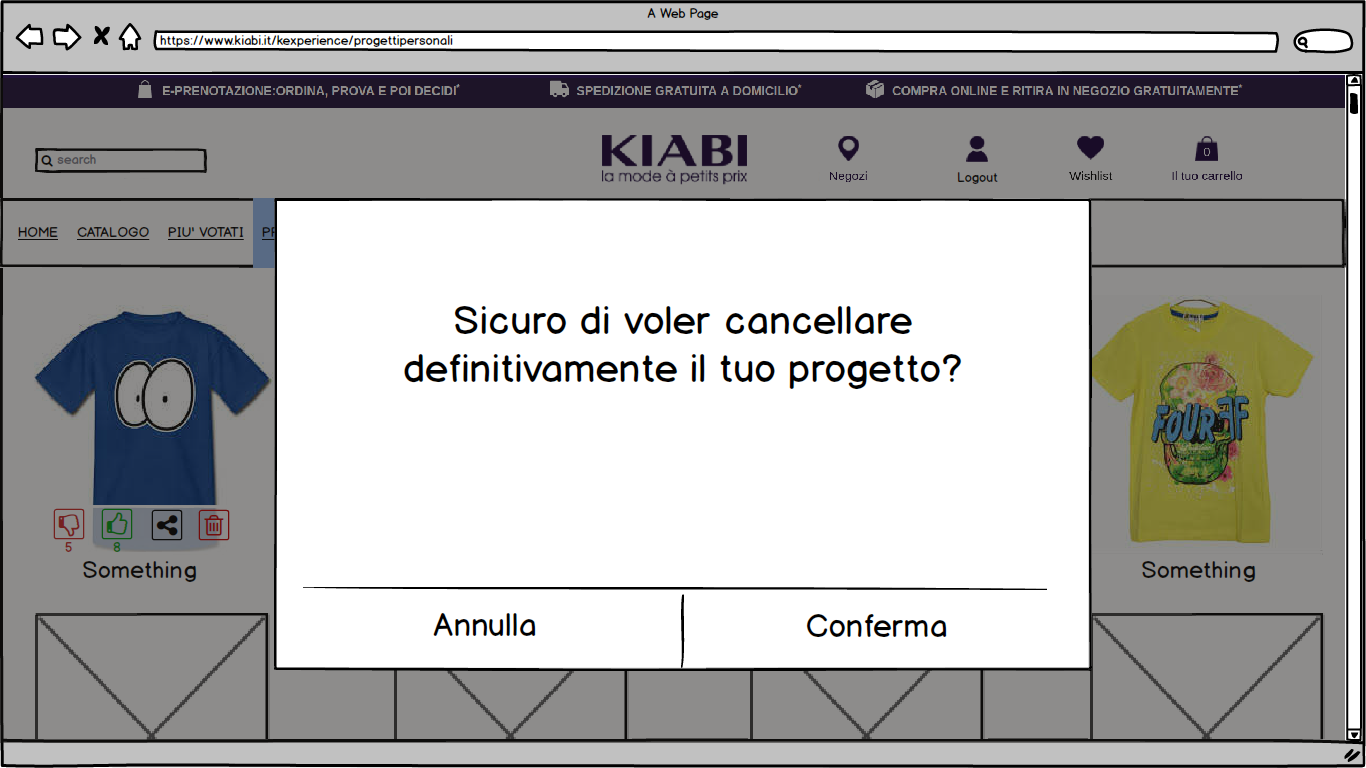
\includegraphics{balsamiq/Progetti Personali eliminazione.png}
\label{progetti_personali_delete}
\caption{Progetti Personali - Modale di eliminaizone}
\end{figure}



\subsection{Progetti più votati} 



La paagina mostra un elenco dei progetti ordinati per differeza tra like/dislike in modo discendente.


\begin{figure}[h]
\centering
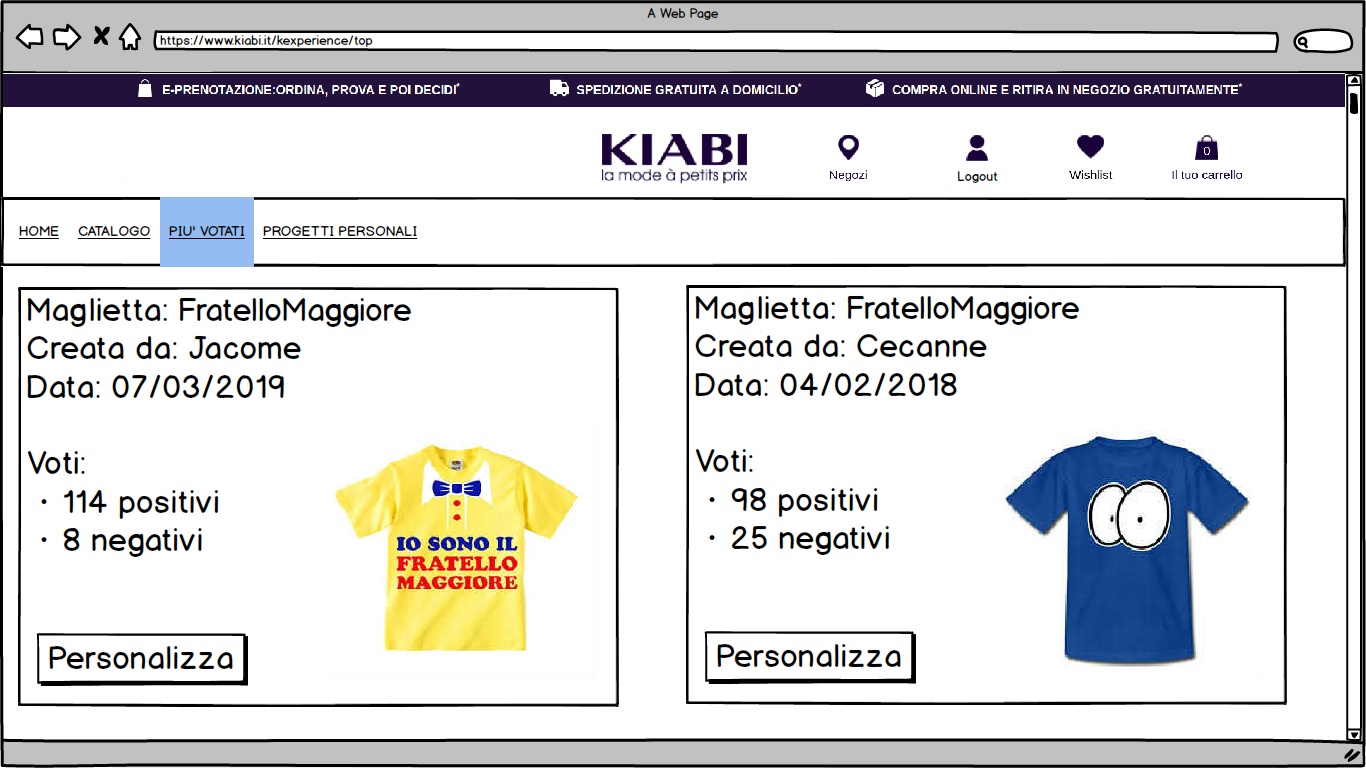
\includegraphics{balsamiq/Most Rated.png}
\label{piu_votati}
\caption{Più Votati}
\end{figure}



\subsection{Editor} 
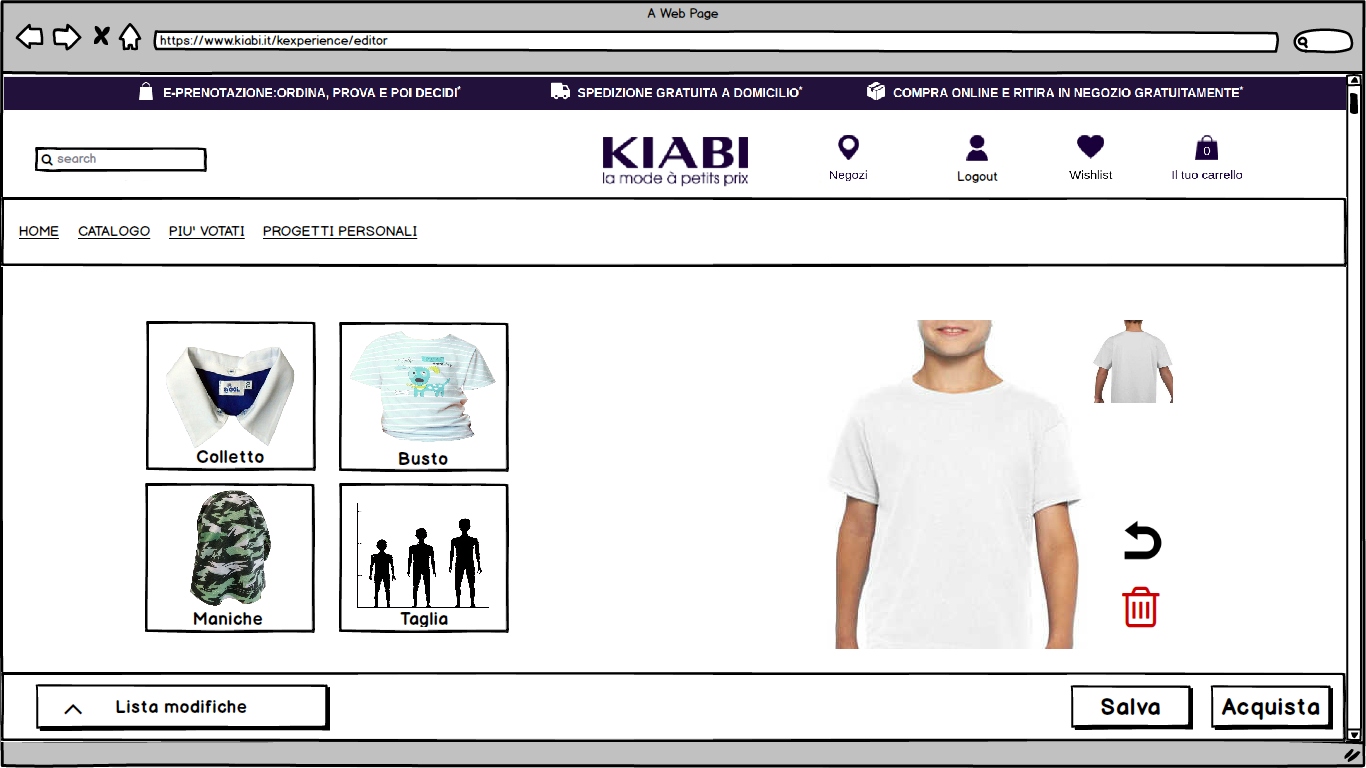
\includegraphics{balsamiq/Editor base.png}


\subsubsection{Salvataggio Progetto} 
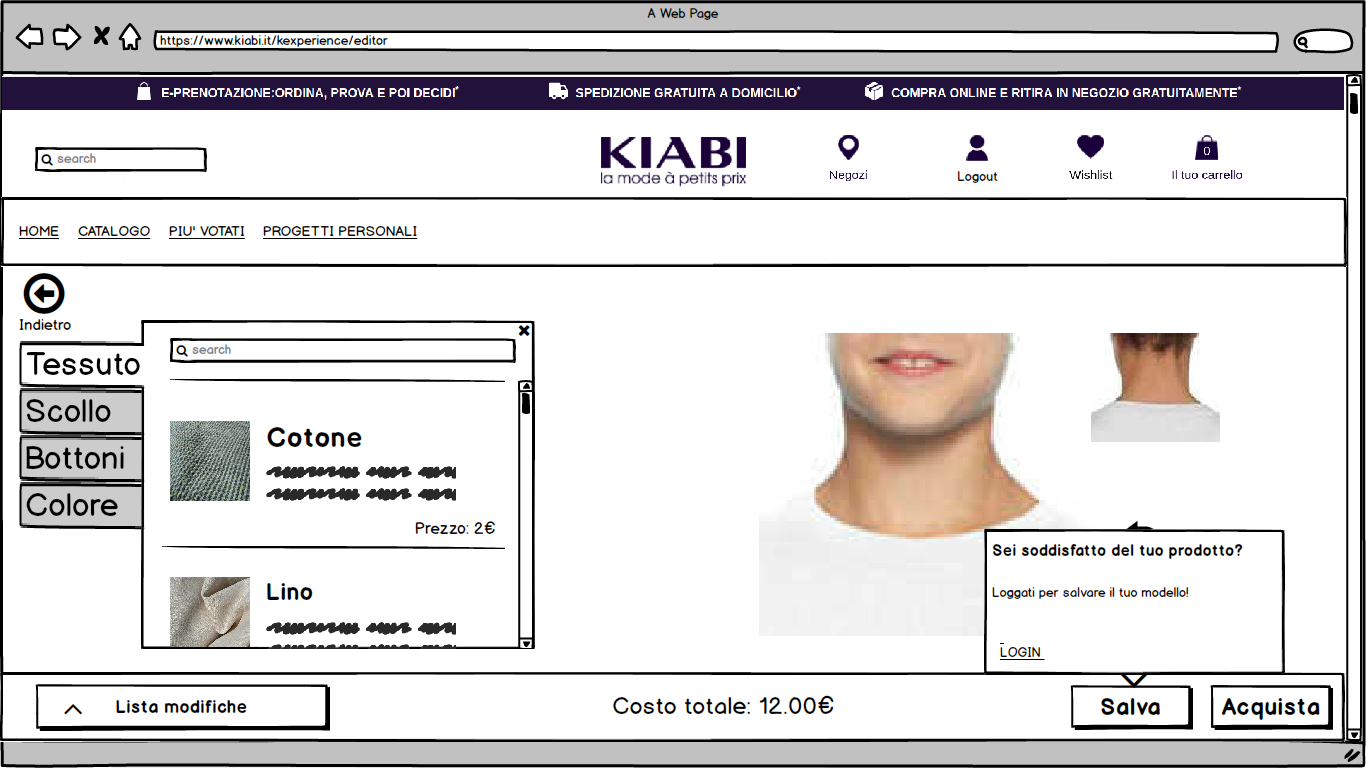
\includegraphics{balsamiq/Editor - caratteristica collo tessuto non loggato.png}

\subsubsection{Editor Colletto} 
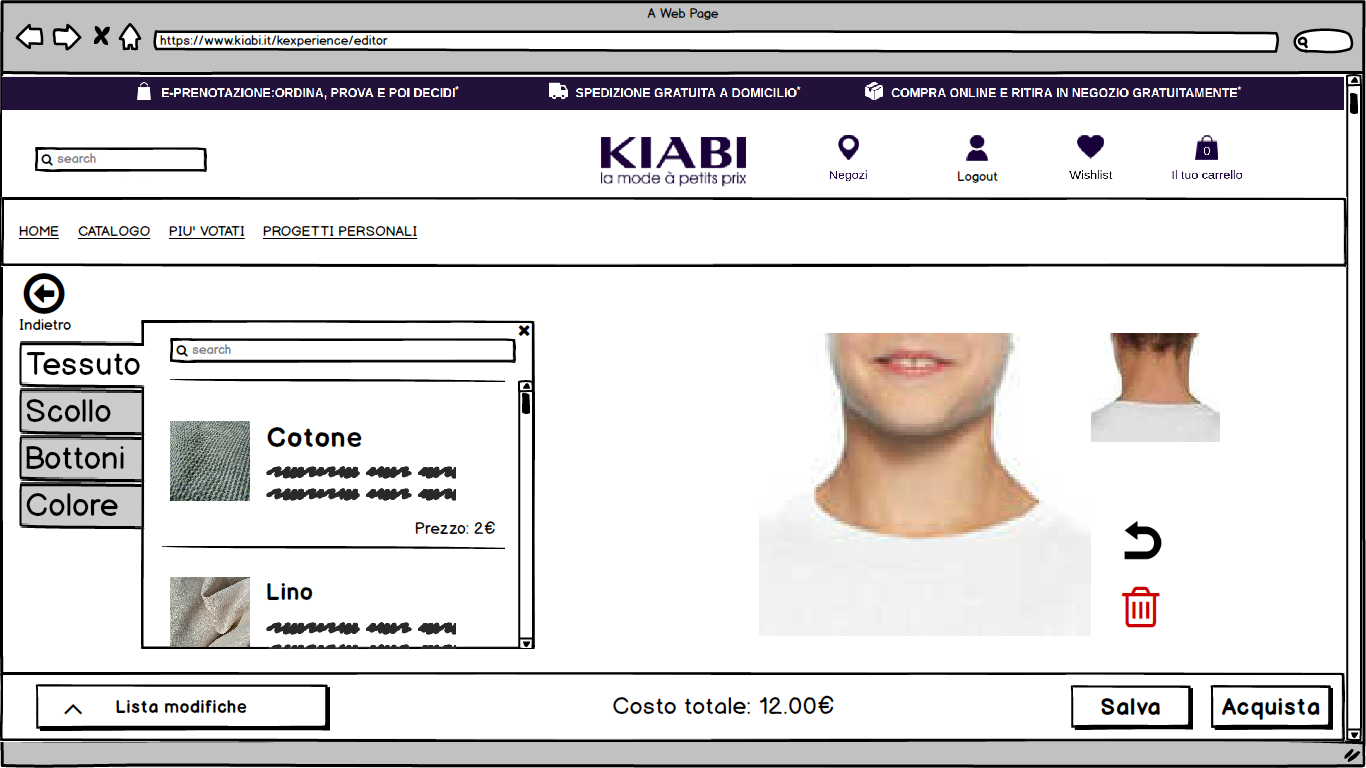
\includegraphics{balsamiq/Editor - caratteristica collo tessuto.png}

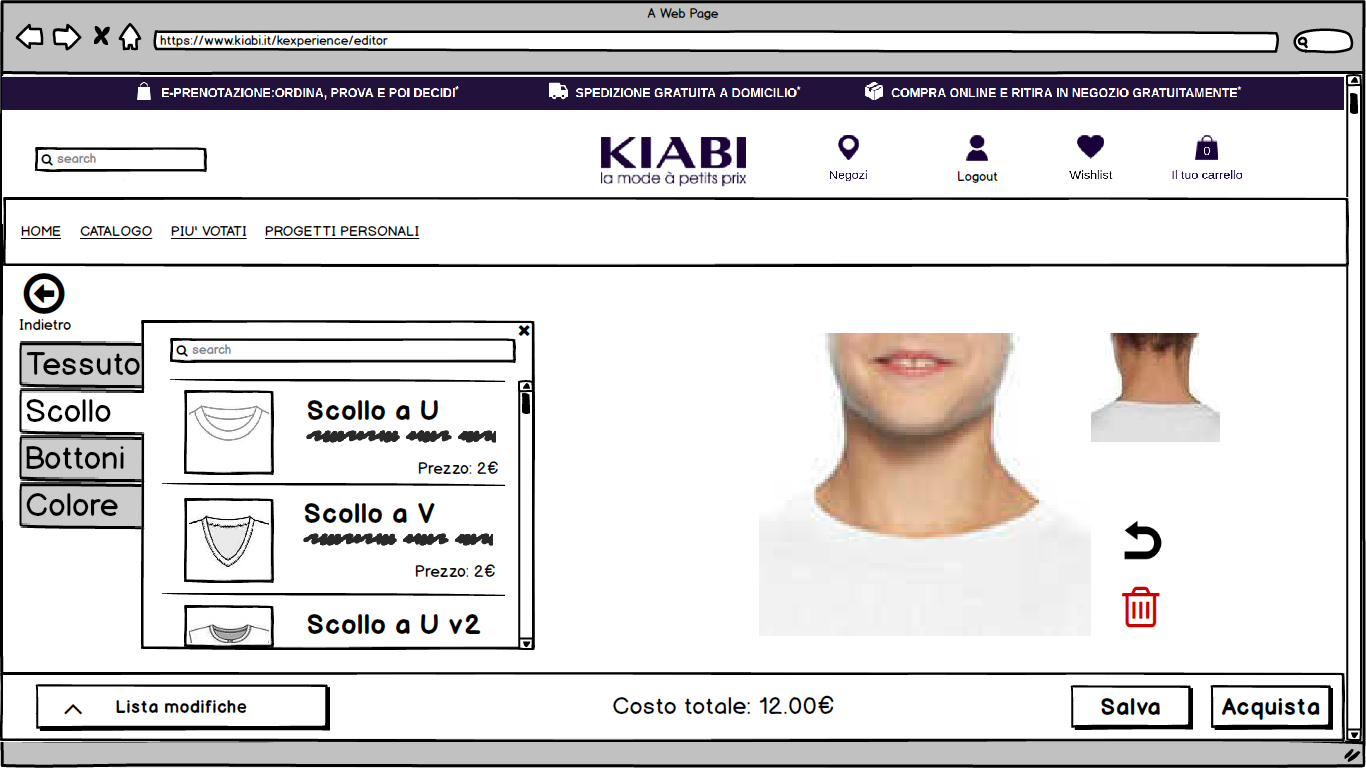
\includegraphics{balsamiq/Editor - caratteristica collo scollo.png}


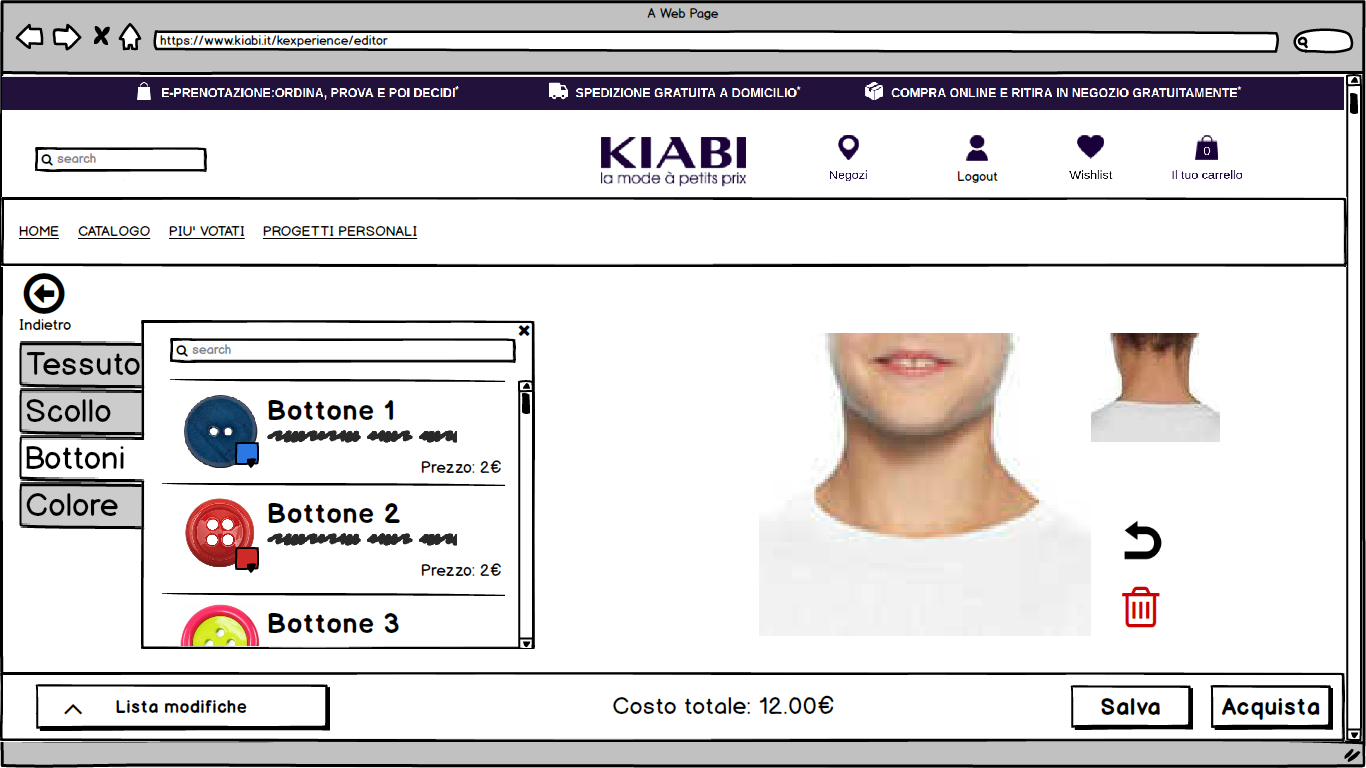
\includegraphics{balsamiq/Editor - caratteristica collo bottoni.png}


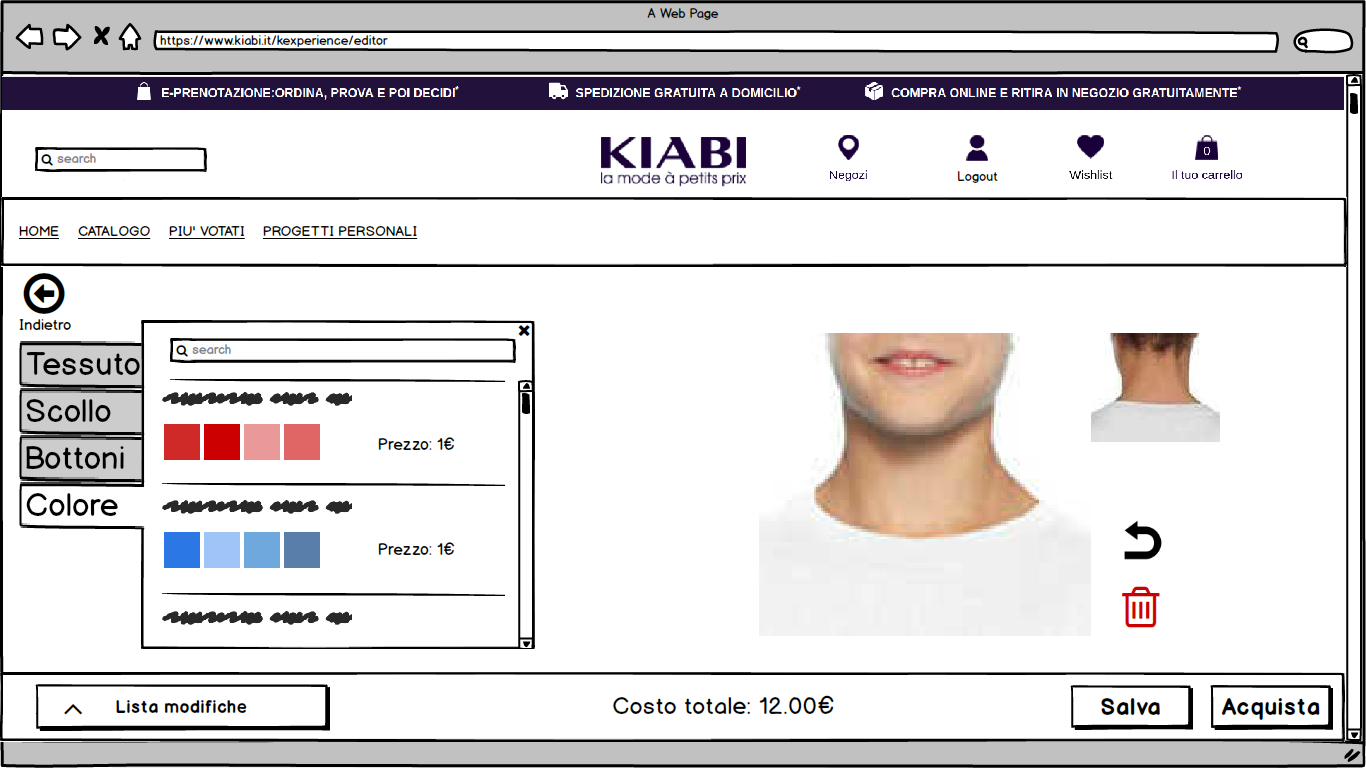
\includegraphics{balsamiq/Editor - caratteristica collo colore.png}


\subsubsection{Editor Busto} 
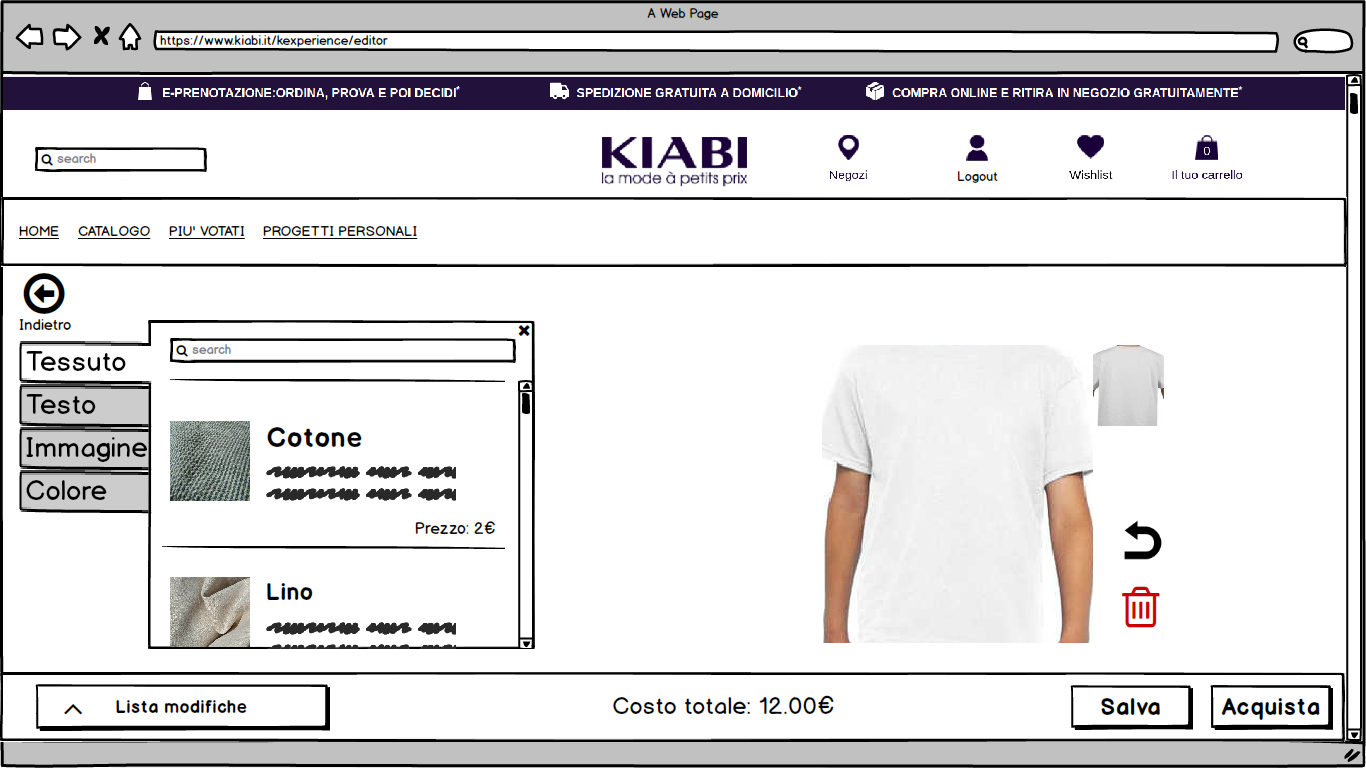
\includegraphics{balsamiq/Editor - caratteristica busto tessuto.png}


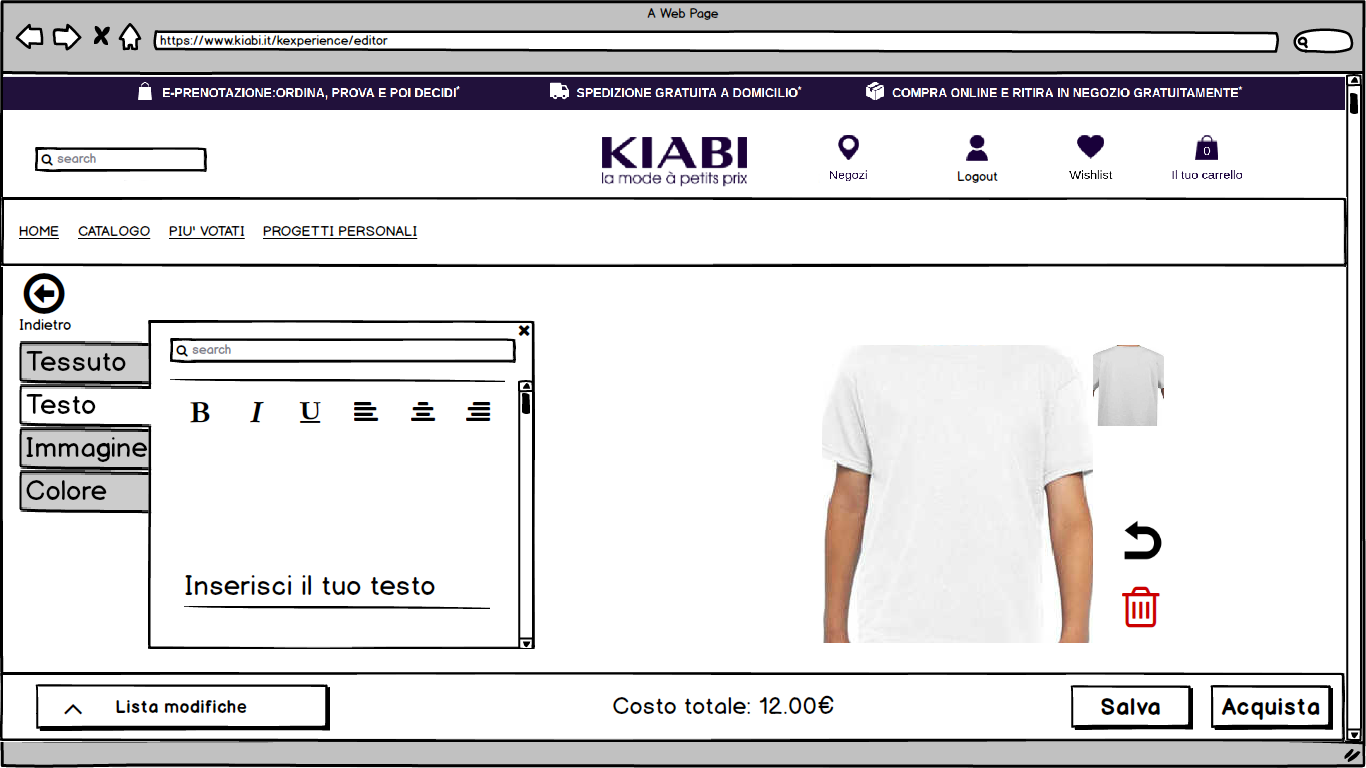
\includegraphics{balsamiq/Editor - caratteristica busto testo.png}


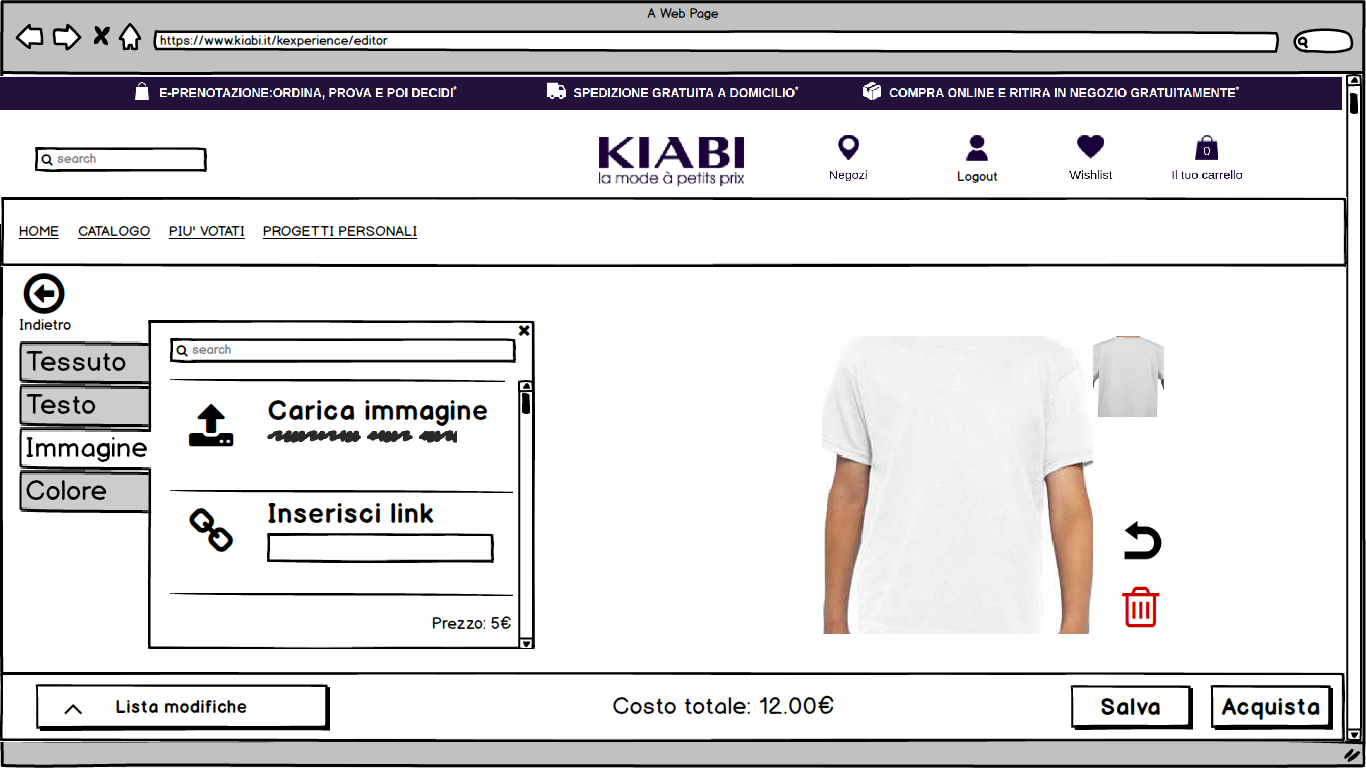
\includegraphics{balsamiq/Editor - caratteristica busto immagine.png}


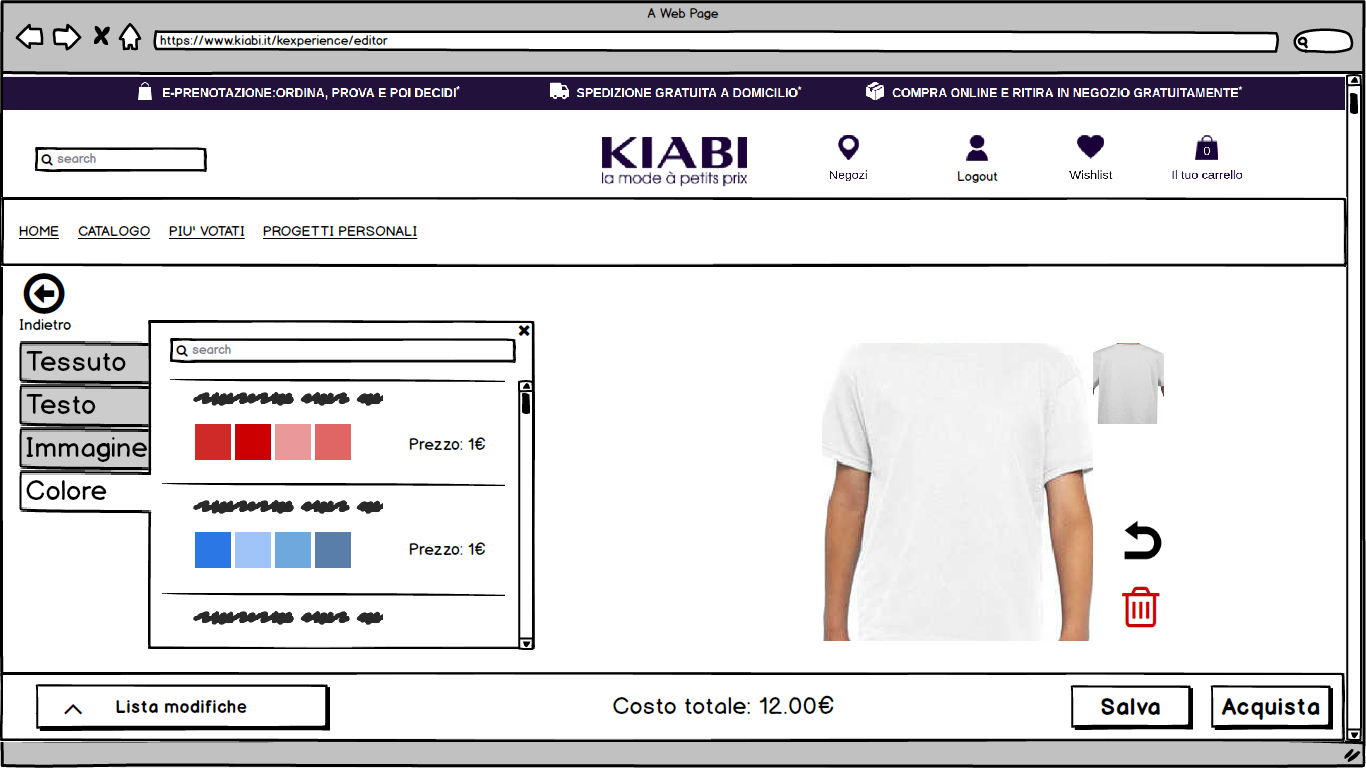
\includegraphics{balsamiq/Editor - caratteristica busto colore.png}
\subsubsection{Editor Maniche} 
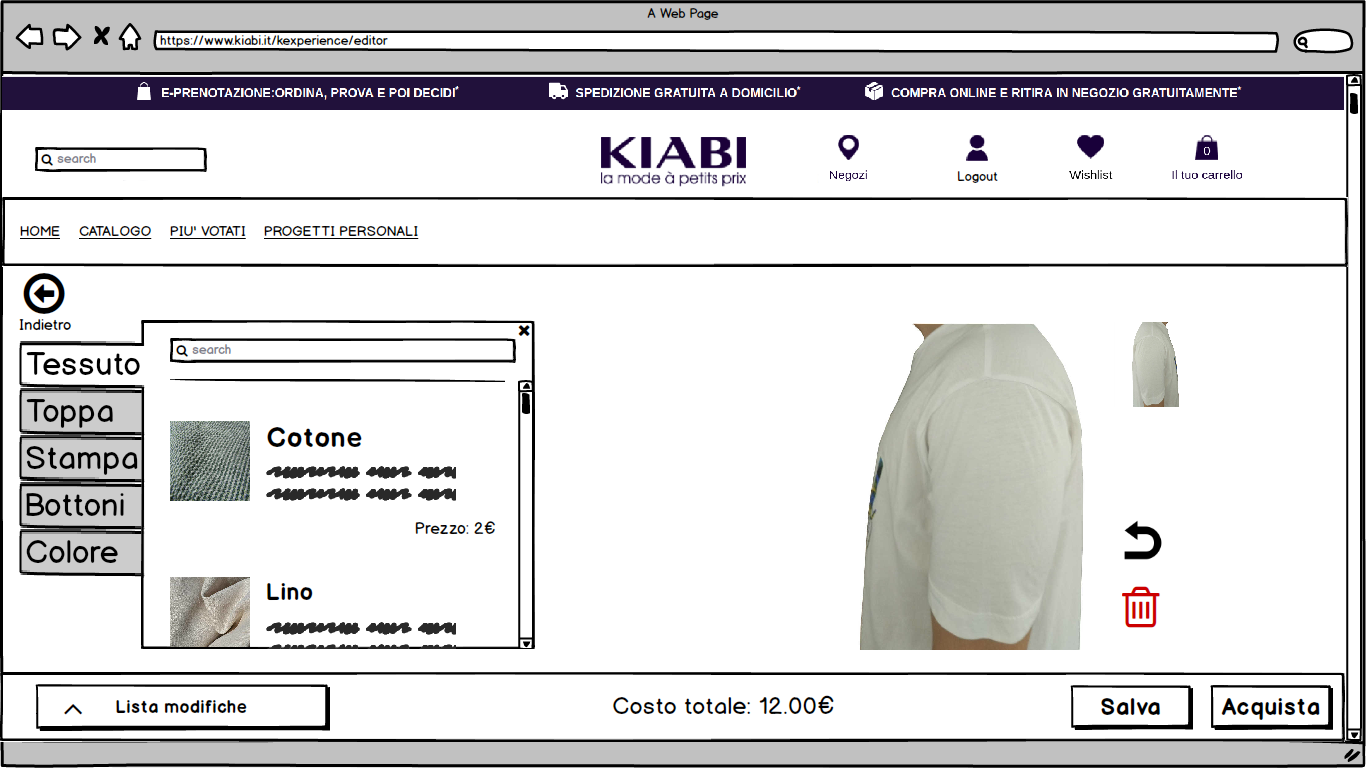
\includegraphics{balsamiq/Editor - caratteristica maniche tessuto.png}


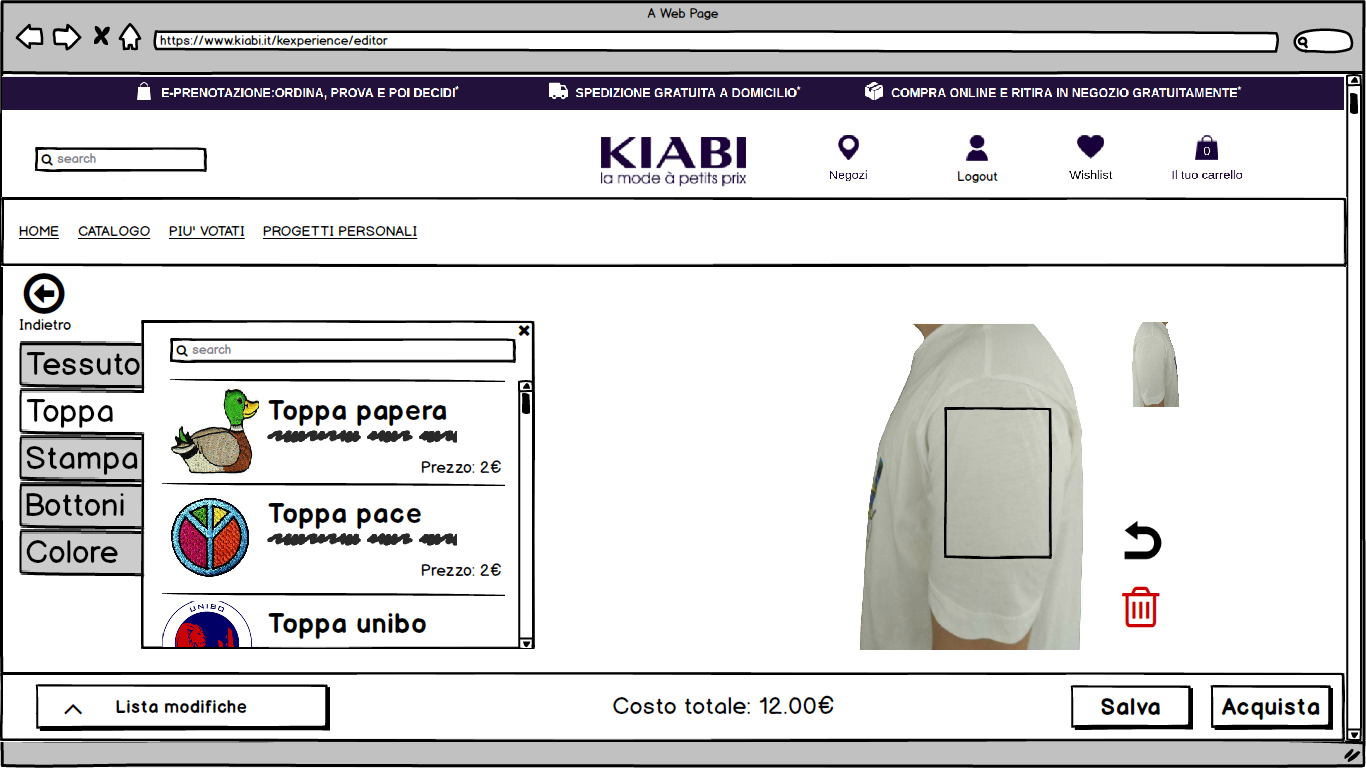
\includegraphics{balsamiq/Editor - caratteristica maniche toppa.png}


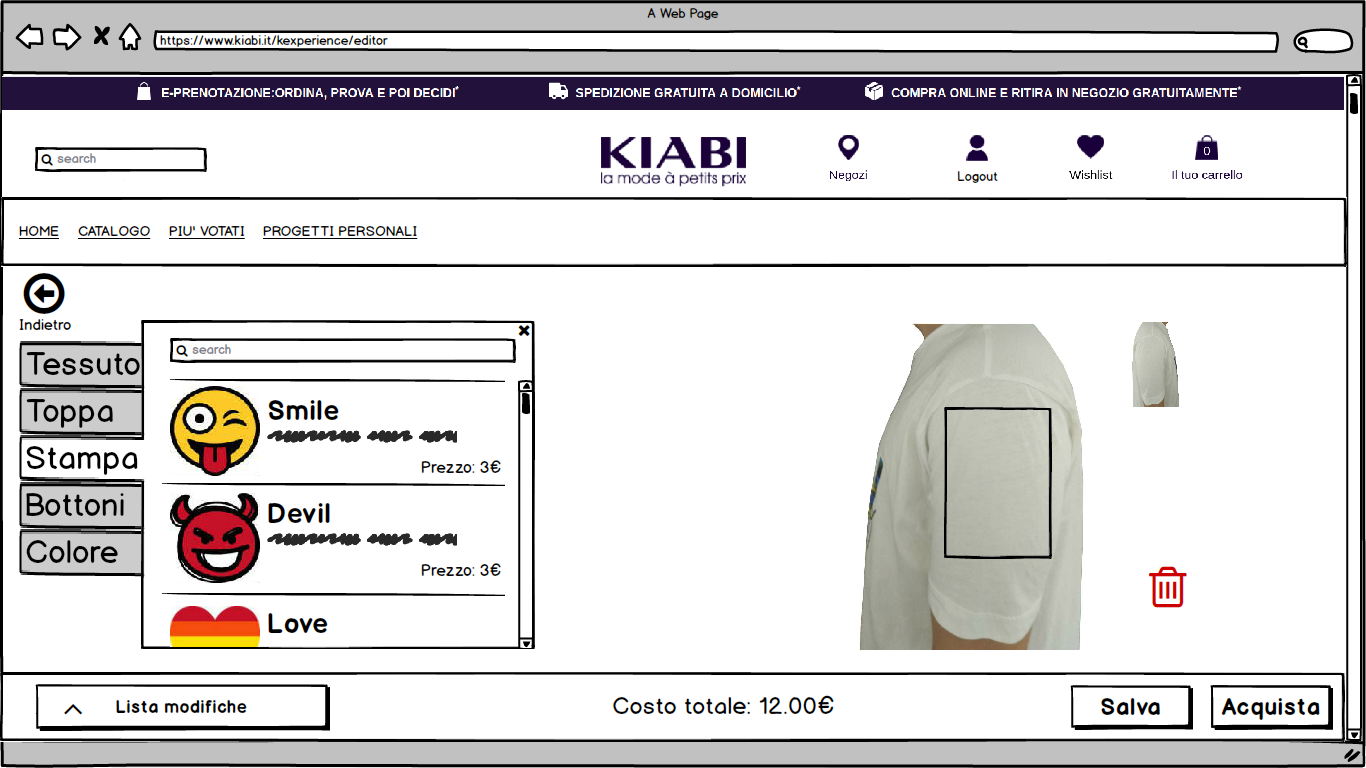
\includegraphics{balsamiq/Editor - caratteristica maniche stampa.png}


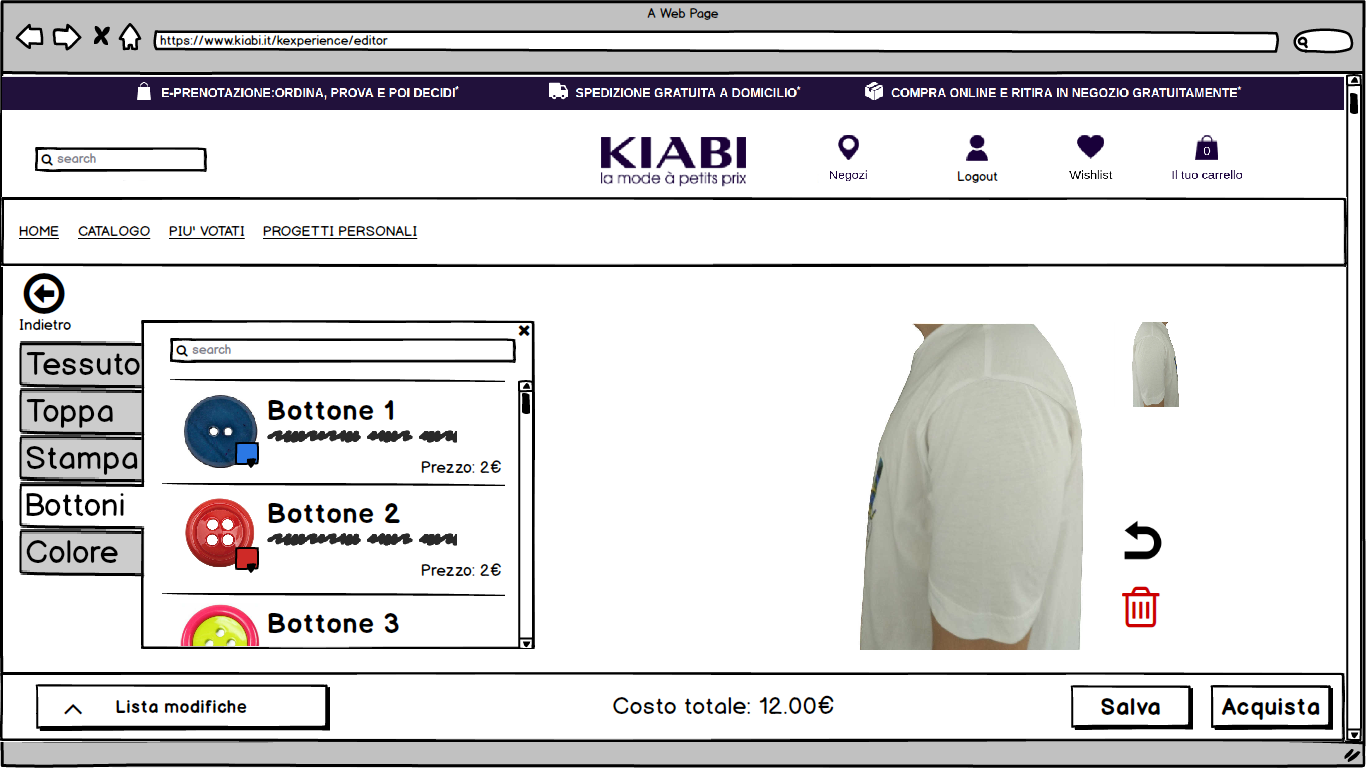
\includegraphics{balsamiq/Editor - caratteristica maniche bottoni.png}


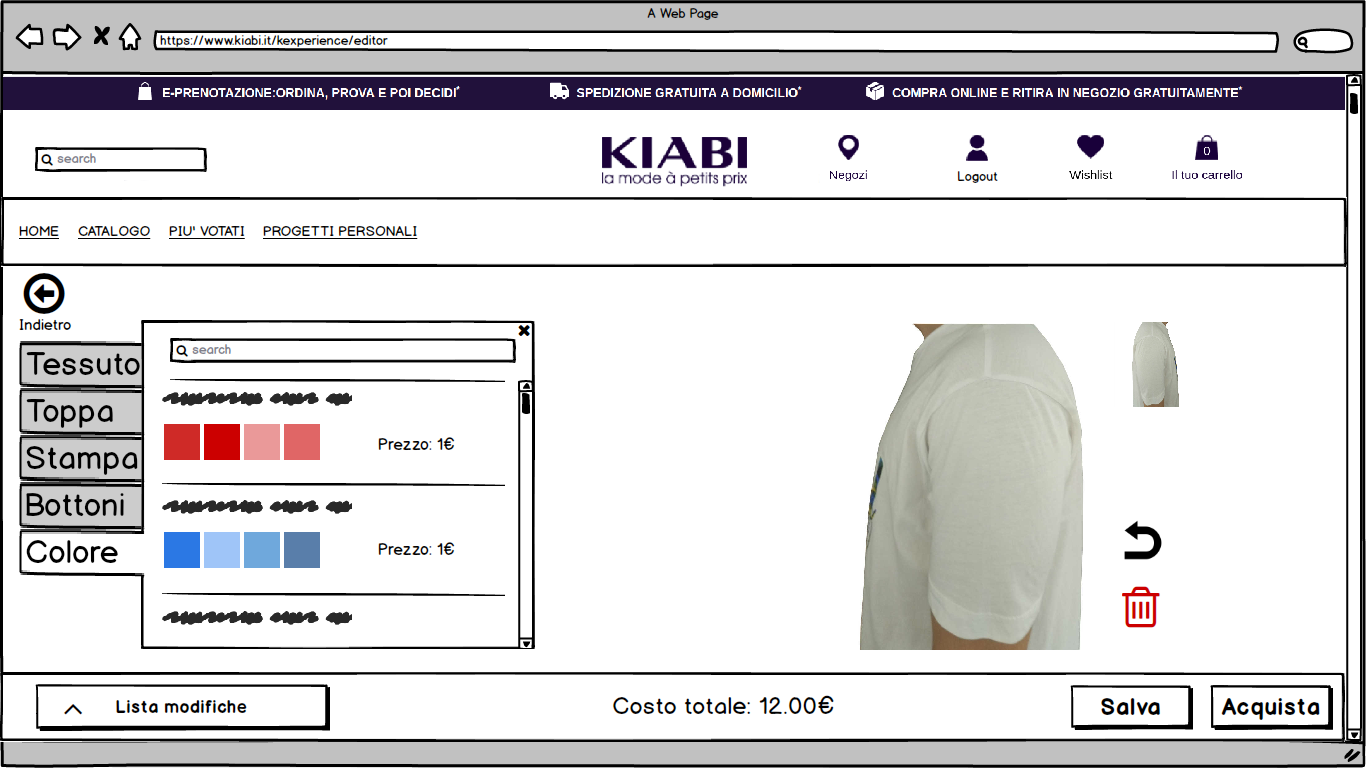
\includegraphics{balsamiq/Editor - caratteristica maniche colore.png}


\subsubsection{Taglia} 
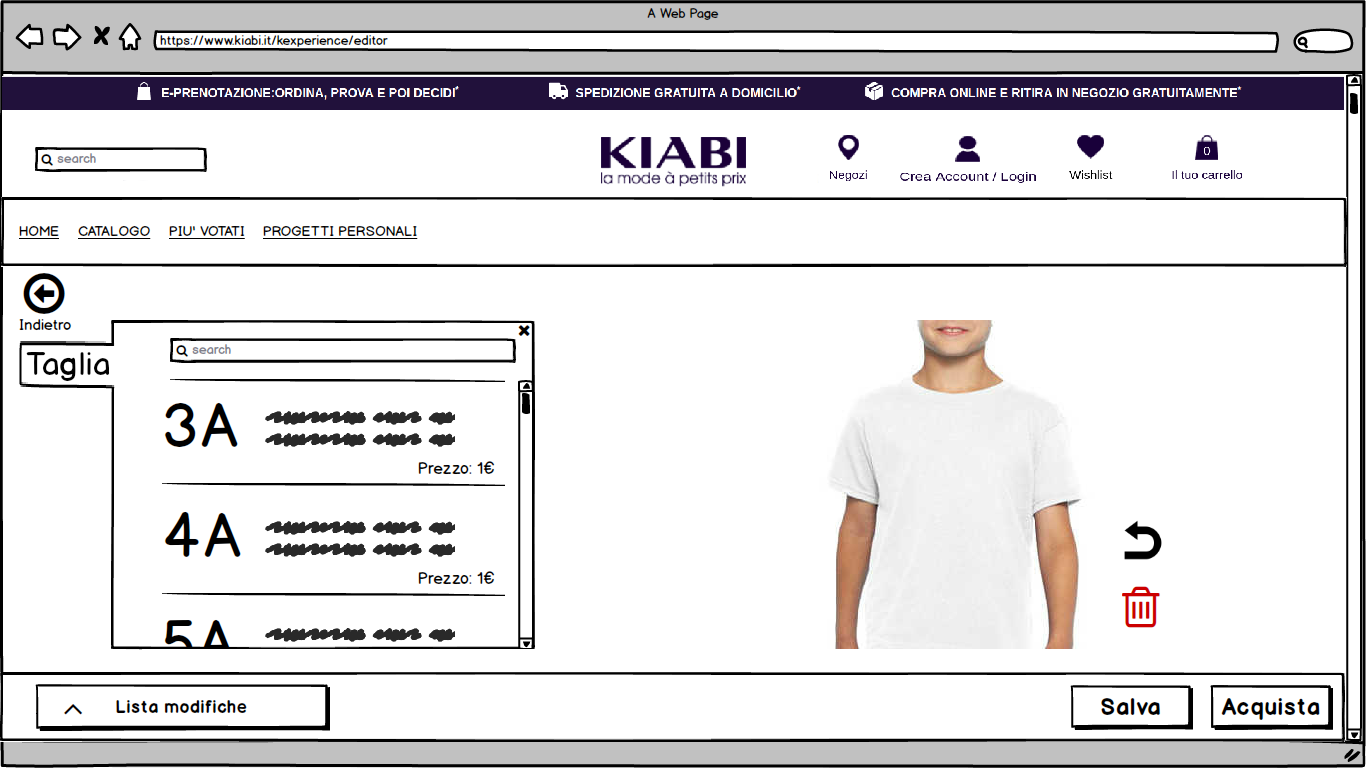
\includegraphics{balsamiq/Editor - caratteristica capo taglia.png}


\subsubsection{Lista Dettagli} 
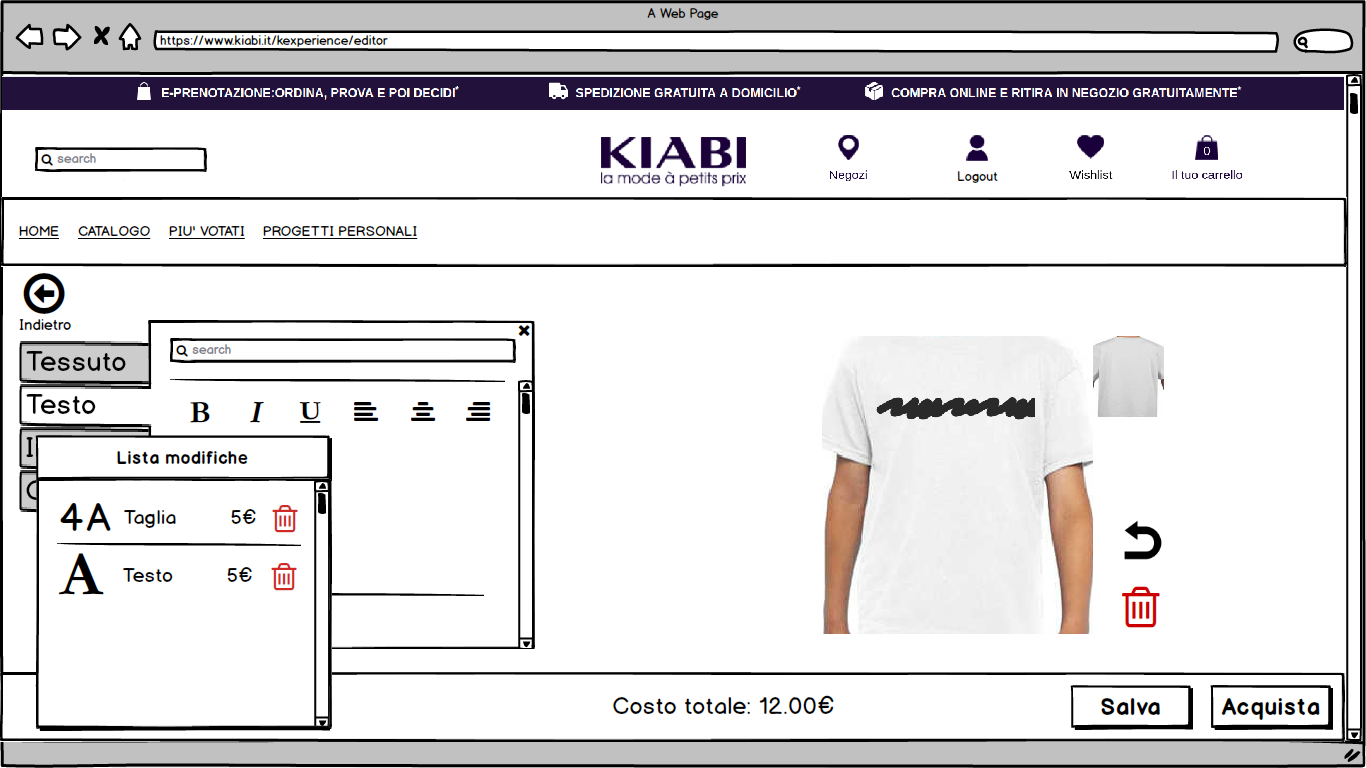
\includegraphics{balsamiq/Editor - caratteristica busto testo 4.png}


\subsection{Carrello} 
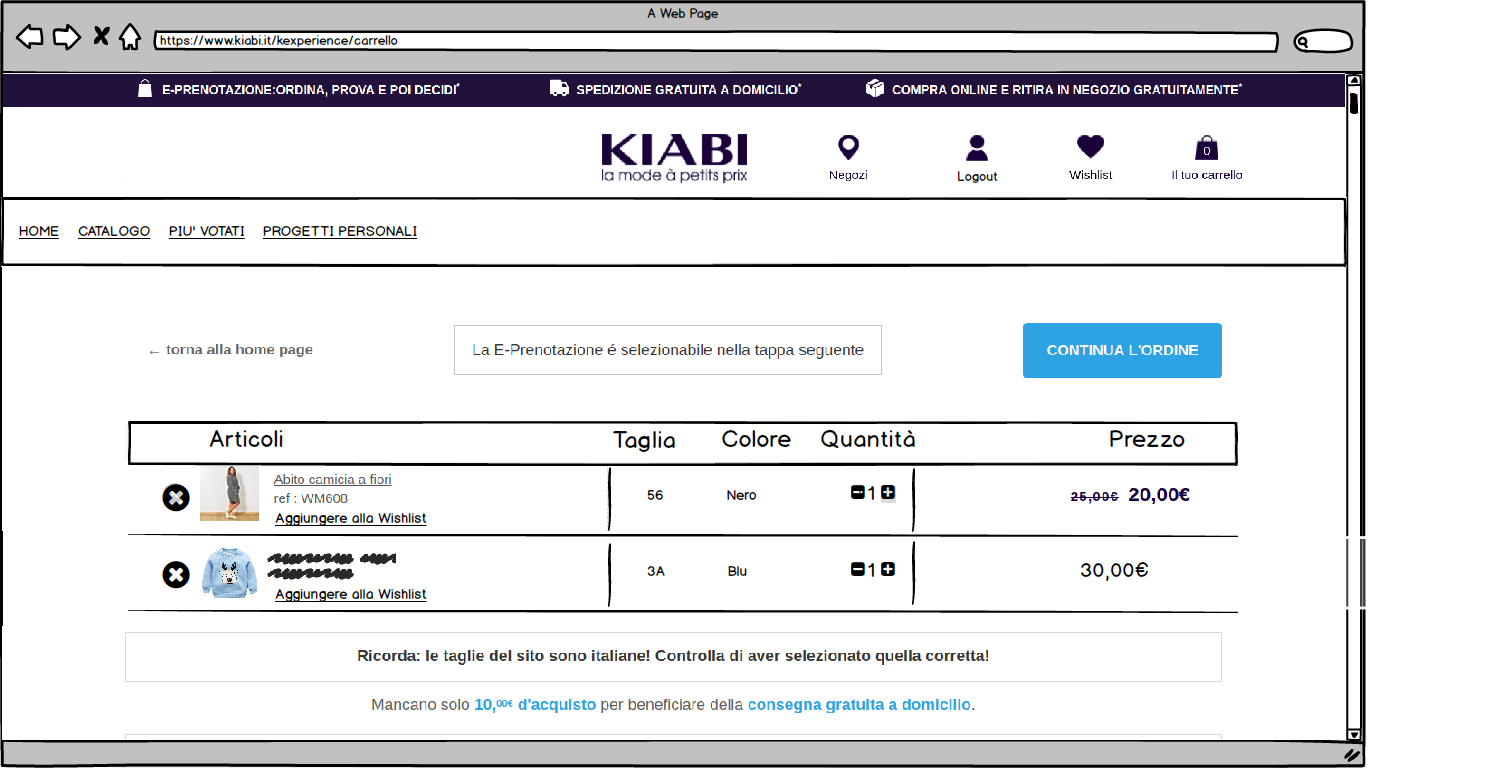
\includegraphics{balsamiq/Carrello.png}


\subsubsection{Dettagli Carrello} 
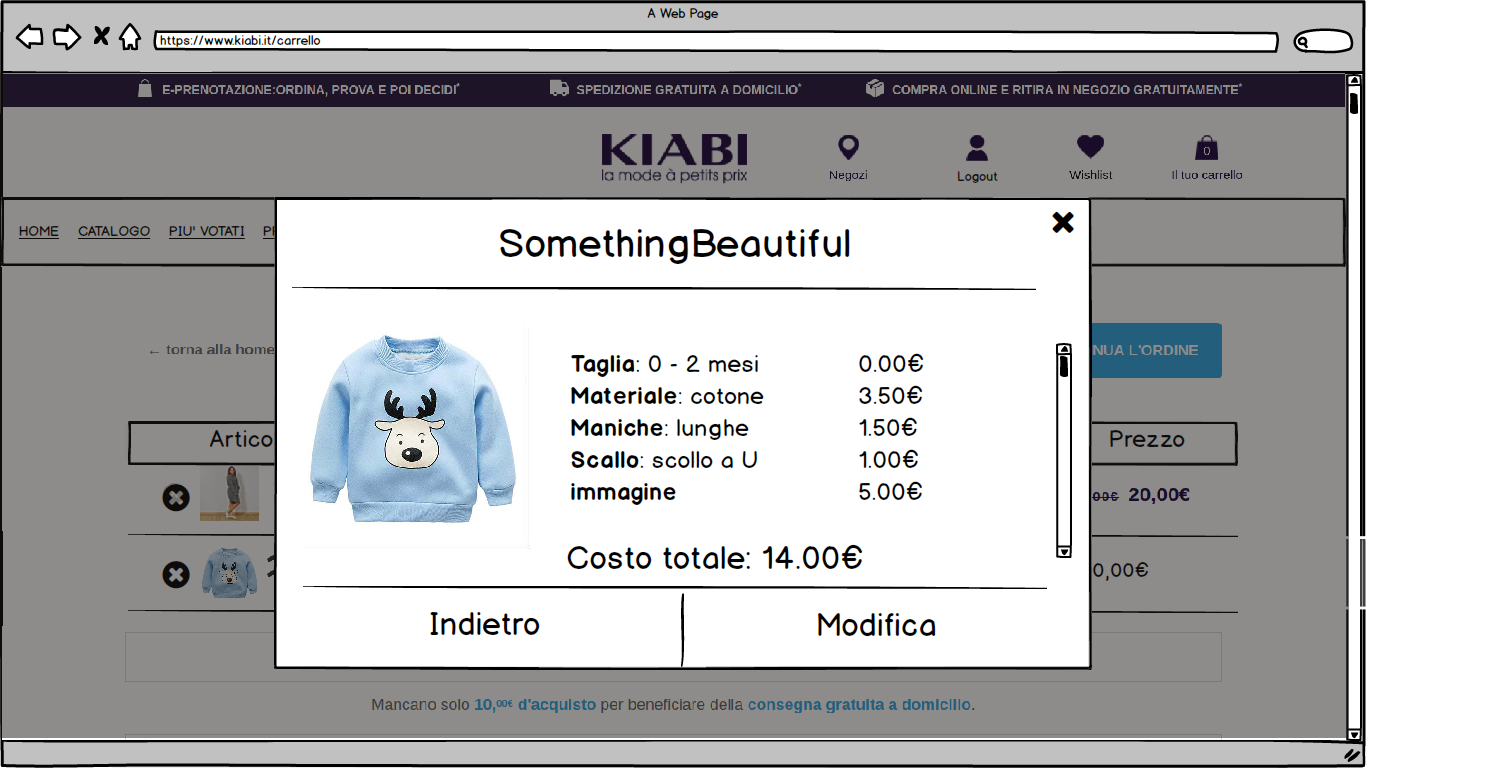
\includegraphics{balsamiq/Carrello dettagli.png}


\subsection{Login} 
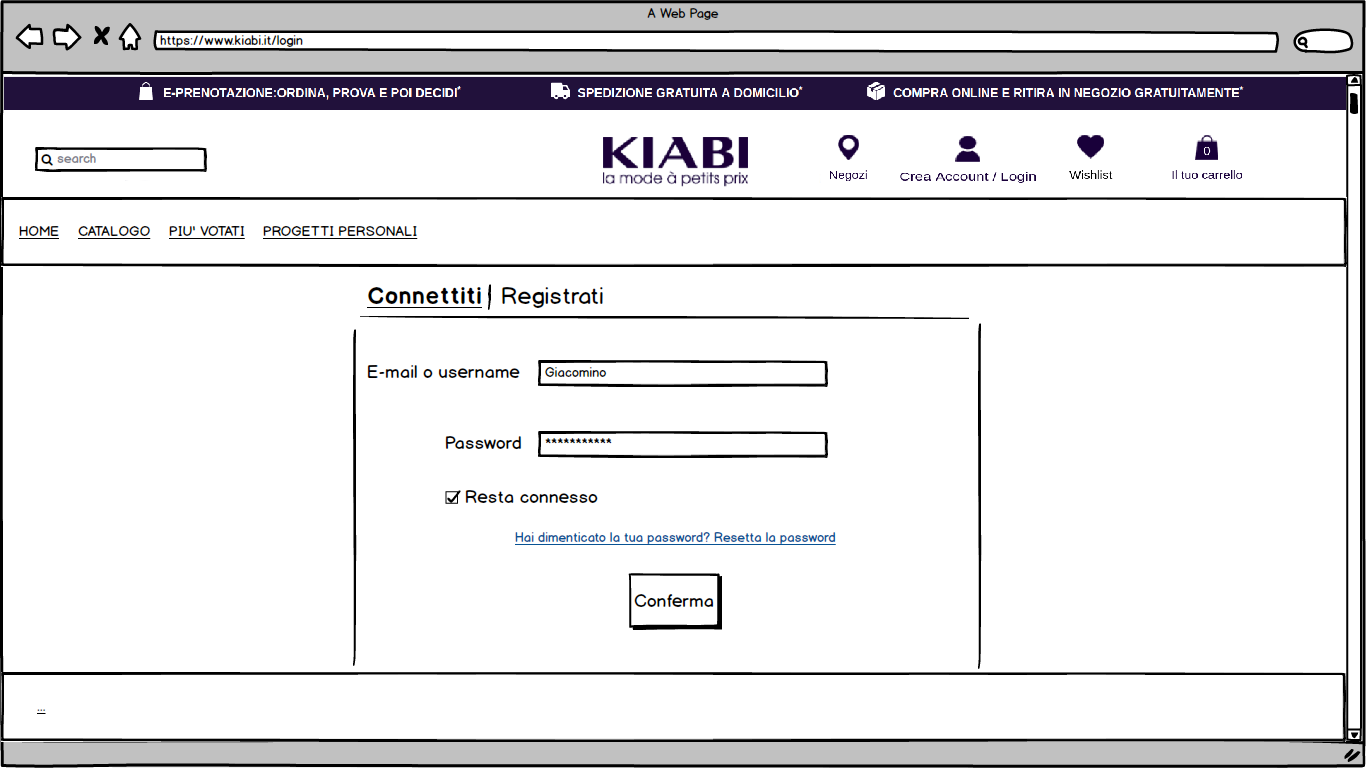
\includegraphics{balsamiq/Login.png}

\subsection{Registrazione} 
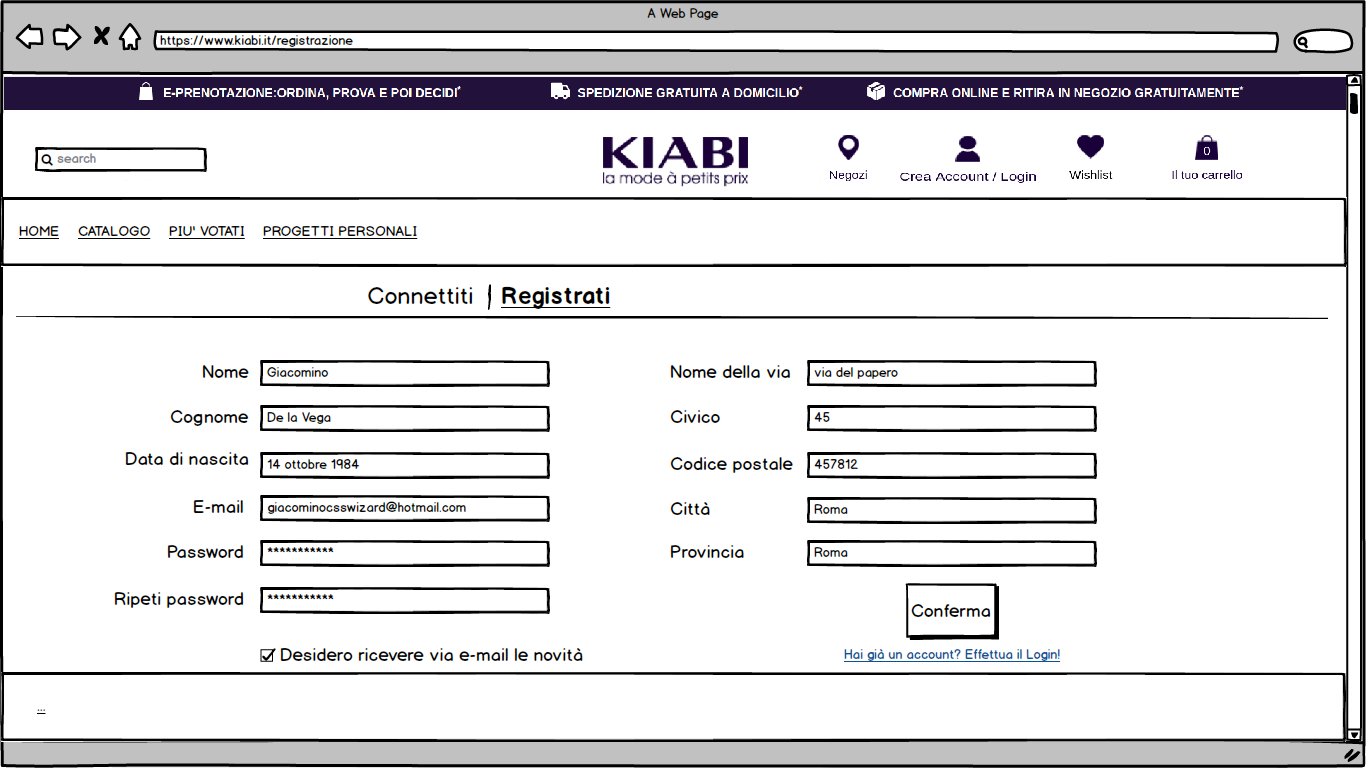
\includegraphics{balsamiq/Registrazione.png}
\end{document}
